\documentclass[a4paper,14pt,twoside
%,draft
]{scrreprt}

\usepackage[parfill]{parskip}
\usepackage{graphicx}
\usepackage{fancyhdr}
\usepackage{eso-pic}
\usepackage{caption}
\usepackage{hyperref}
\usepackage{wrapfig}

\usepackage{fontspec}
\usepackage{polyglossia}
\setmainlanguage{german}
\newcommand{\glqq}{„}
\newcommand{\grqq}{“}

\definecolor{ifsrgreen}{rgb}{0.69, 0.88, 0.11} % 177, 225, 28
\definecolor{ifsrgray}{rgb}{0.6, 0.6, 0.6} % 153, 153, 153

\setmainfont{PT Sans}
\setkomafont{chapter}{\color{ifsrgreen}\fontspec[BoldFont={* Bold}]{Exo}\huge}
\setkomafont{chapterentry}{\normalfont\bfseries}
\setkomafont{minisec}{\color{ifsrgray}\fontspec[BoldFont={* Bold}]{Exo}\large}
\setkomafont{paragraph}{\color{ifsrgray}\fontspec[BoldFont={* Bold}]{Exo}}
\setkomafont{pagenumber}{\color{ifsrgray}\fontspec{Roboto}}

\sloppy % forces "ugly" line breaks

\pagestyle{plain}

%Das Coverbild, oh gott o.O Aber es funktioniert
\newcommand\CoverPic{%
\put(0,0){%
\parbox[b][\paperheight]{\paperwidth}{%
\vfill
\centering
\includegraphics[width=\paperwidth,height=\paperheight,%
keepaspectratio]{img/cover_2014}%
\vfill
}}}

%Das Rückbild, den Text können wir aber nach wie vor hier direkt reinschreiben, erzeugen wir einfach ne leere farbige Rückseite.
\newcommand\BackcoverPic{%
\put(0,0){%
\parbox[b][\paperheight]{\paperwidth}{%
\vfill
\centering
\includegraphics[width=\paperwidth,height=\paperheight,%
keepaspectratio]{img/backcover_old.png}%
\vfill
}}}

\begin{document}

\thispagestyle{empty} %keine Seitenzahl
\AddToShipoutPicture*{\CoverPic}
\mbox{} %brauche leeren Content für ne newpage
%\newpage

\tableofcontents
\textbf{Danke an ...}
\\

\begin{tabular}{l l l} 

Jakob Blume & Ulrich Huber & Mike Pohl\\
Anika Borchmann & Sönke Huster & Axel Reinicke\\
Anna Brauer & Christian Kabelitz & Franziska Ressel\\
Thomas Bruhn & Christoph Kepler& Marcel Rösler\\
Markus Damm & Maximilian Kindt & Simon Rother\\
Jasmin Delling & Clemens Köhler & Marc Satkowski\\
Felix Döring & Kilian Költzsch & Michael Schneider\\
Lars Engeln & Max Korn & Sebastian Schrader\\
Niklas Fallik & Ben Kosmann & Franz-Wilhelm Schumann\\
Paul Genssler & Alexandra Krien & Lara von Schumann\\
Bettina Groschopp & Raphael Lais & Max Staff\\
Anita Grützner & Dirk Legler & Patrick Stiller\\
Lukas Haack & Adrian Lieber & Manuel Thieme\\
Sebastian Hahn & Katja Linnemann & Lucas Vogel\\
Simon Hanisch & Ian Alexander List & Sebastian Vogt\\
Thomas Hauptvogel & Sebastian Mielke & Tilo Werdin\\
Frank Hedecke & Richard Mörbitz & Jens Wettlaufer\\
Joschka Heinrich & Michael Nix & Jan-Erik Wieczorek\\
Philipp Heisig & Dominik Olwig & Felix Wittwer\\
Robin Herrmann & Sascha Peukert & Lucas Woltmann\\

\end{tabular}

\addchap{Vorwort}

Hallo Uniwelt!

heißt es nun für dich als frisch Immatrikulierter, Ersti, an der TU Dresden. 
Endlich kannst du nach Jahren der Knechtschaft selbst über dich und dein Leben bestimmen. 
Wie du mit dieser Freiheit und der daraus folgenden Verantwortung zurecht kommst, lernst du schnell. 
Damit dir der Übergang leichter fällt, veranstaltet dein Fachschaftsrat die Erstsemestereinführung (ESE). 
Eine Woche lang gibt es neben Spiel und Spaß sehr viel Informatives zum Studium sowie zum Unileben allgemein. 
Dieses Heft ist ein nützlicher Ratgeber und nicht vergessen: 
\textbf{NO PANIC!} (Aus historischen Gründen hier nicht das grammatikalisch korrekte \glqq don't panic\grqq.)

Du wirst auch entdecken, dass Uni mehr ist als nur studieren. 
Neben allerlei Erstsemesterparties gibt es noch mehr zu erleben. 
Gerade prägend für die Dresdner Hochschulkultur sind die 16 Studentenclubs, wie z.B. das CountDown in der Johannstadt. 
In der Neustadt laden ebenso viele Kneipen und Clubs zu langen Nächten ein. 
Einmal im Jahr entlädt sich dieses alternative Flair während der BRN (Bunte Republik Neustadt). 
Und wem das alles viel zu hektisch ist: der fläze sich gemütlich in ein Sofa vom ASCII, dem Studentencafé der Fakultät. 
Dort kann man gut bei Kaffee und Club Mate (empfehlenswert auch die lokale Kolle-Mate!) entspannen oder versuchen doch etwas für die Uni zu tun.

Engagement wird an der TU Dresden groß geschrieben. 
Es gibt viele Hochschulgruppen die um eure Mitarbeit buhlen. 
Darunter einige politische, wie auch technische, journalistische, künstlerische und und und. Mehr dazu findest du auf der Seite des Studentenrates (StuRa).

Dieses Heft enthält übrigens auch eine Vielzahl von Links zu relevanten Unterseiten auf den Seiten des Fachschaftsrates (FSR), der Uni und anderen. 
Diese sind mit Zahlen wie dieser hier \link{https://html5zombo.com} versehen und ganz am Ende des Heftes gelistet. Ebenfalls kannst du auch direkt unter \url{ese.ifsr.de/2015/<Zahl>} auf die verlinkte Seite weitergeleitet werden.

\textbf{Zu guter Letzt: Wir (deine ESE-Tutoren) wünschen dir viel Erfolg und auch ordentlich Spaß beim Studium!}

\thispagestyle{empty}
\AddToShipoutPicture*{\put(0,0){%
\parbox[b][\paperheight]{\paperwidth}{%
\vfill
\centering
\refstepcounter{dummy}
\label{we_want_you}

\includegraphics[width=\dimen107,height=\dimen108,keepaspectratio]{img/we_want_you.jpg}%
\vfill
}}}
\ 
\pagebreak

\addchap{Grußwort}

\begin{wrapfigure}{l}{0.31\textwidth}
  \vspace{-12pt}
  \begin{centering}
    \includegraphics[width=0.3\textwidth]{img/uweassmann.png}
  \end{centering}
  \vspace{-15pt}
\end{wrapfigure}

{\fontsize{9.5pt}{11}\selectfont

Liebe Studierende,

herzlichen Glückwunsch zum Beginn eines der spannendsten Studien, die es gibt, an einer der attraktivsten Informatikfakultäten Deutschlands und Europas! Als Dekan ist es mir eine Freude, Sie herzlich an unserer Fakultät Informatik begrüßen zu dürfen. Mit 26 Professoren, 3 Honorarprofessoren, mehr als 300 Mitarbeitern und mehr als 1600 Studenten gehört die Fakultät zu den größten Informatikfakultäten Deutschlands mit einem der breitesten Spektren an Studieninhalten. Um unser modernes Gebäude werden wir von vielen anderen Fakultäten beneidet, auch wenn es manchmal mit einem Augenzwinkern als "Grünes Gewölbe" bezeichnet wird. Ich kann Ihnen aus eigener Erfahrung versichern: man gewöhnt sich an die Farbe. Das Gebäude bietet nicht nur Platz für die Mitarbeiter der Fakultät, sondern verfügt auch über einen Vorlesungssaal, diverse Seminarräume und hochwertig ausgestattete Rechner-Pools. Im Foyer liefert das Studentencafé \ascii{} den für einen Wissenschaftsbetrieb äußerst wichtigen Koffeinnachschub. Was unser Kunstwerk im Atrium bedeutet, dürfen Sie gerne raten. Hinter unserem Gebäude lädt das "Nöthnitzer Meer" zum Lernen, Chillen und Sonnen ein. Und gleich links von der Fakultät liegt unser beliebtes Sportzentrum.

Die Informatik durchdringt unsere Gesellschaft wie keine andere Wissenschaft und beschleunigt den wissenschaftlichen Fortschritt anderer Disziplinen enorm. Marc Andreesen, der Erfinder des ersten kommerziellen Web-Browsers "Netscape", prägte in 2011 den Slogan "Software is eating the world", was sagen will, dass die Digitalisierung alle Industrien und alle Lebensbereiche verändert. Software läuft nicht nur in Computern, sondern auch in Autos, Flugzeugen, Wasch- und Kaffeemaschinen. Teilweise ist der Einfluss von Software sogar so tief, dass er der Gesellschaft gar nicht mehr bewusst ist: Wer denkt heute schon darüber nach, dass sein Handy aus einem Berg voller Software besteht? Die Digitalisierung führt auch dazu, dass Firmen händeringend nach Informatikern suchen. Unsere Fakultät kann derzeit mit ihren Absolventen nicht einmal den Fachkräftebedarf der Software-Industrie im Raum Dresden decken, denn sie wächst jedes Jahr um ca. 5-7\% und benötigt dazu ca. 600 neue Informatiker. Nach dem erfolgreichen Abschluss Ihres Studiums werden Ihnen daher viele Türen offenstehen. Also zunächst einmal herzlichen Glückwunsch zu diesen guten Aussichten!

Für Sie, liebe Studentinnen und Studenten, beginnt mit dem Studium ein neuer, faszinierender Lebensabschnitt, der mehr Freiheiten bietet als die Schule vorher und das Berufsleben danach. Diese Freiheiten sollten Sie nutzen, um sich in freier Selbstbestimmung zu bilden, Ihr Studium selbst zu planen, Ihre Lerninhalte selbst zu vertiefen und sich selbst Ihre Lern-Arbeit einzuteilen. Das macht Spaß -- es bringt aber auch zwei Probleme mit sich: Erstens muss man das systematische Erarbeiten von großen Mengen an Lernstoff trainieren, und zweitens benötigt man für ein erfolgreiches Studium mehr Disziplin, als man von der Schule gewohnt ist. Also, einige Tipps: Gehen Sie bitte regelmäßig in die Vorlesungen, denn der Professor fasst dort für Sie die wichtigsten Inhalte des Fachgebiets zusammen, sodass Sie schnell Wichtiges von Unwichtigem unterscheiden können. Bereiten Sie bitte diese Kerninhalte Ihres Faches regelmäßig nach, denn dann verankern sie sich schneller in Ihrem Kopf -- nichts ist schlimmer als eine Woche Bulimie-Lernen vor der Prüfung. Schließlich: Erarbeiten Sie sich die Lösungen zu den Übungsaufgaben selbstständig, denn das selbstständige Lösen von Aufgaben führt Sie schnell zu einer höheren Stufe des Lernens und der damit verbundenen Leistungsfähigkeit (Bloomsche Lernzielhierarchie, siehe Wikipedia). Das erfolgreiche Herunterladen der Vorlesungsfolien oder des Skripts zur Vorlesung trägt nur dann zum Bestehen der Prüfung bei, wenn Sie sich auch intensiv mit den Inhalten auseinandersetzen :-) Versuchen Sie, alle Begriffe zu verstehen und zusätzlich in der Lage zu sein, sie aktiv erklären zu können. Laden Sie sich gegenseitig zum Kaffee ins \ascii{} ein und erklären Sie sich dabei, was in der letzten Vorlesung behandelt worden ist.  Das verbessert nicht nur den Studienerfolg, sondern macht auch viel mehr Spaß. (Das habe auch ich in meinem Studium so erlebt.) Und wenn Sie trotzdem im Studium auf Probleme stoßen, stehen Ihnen viele Anlaufstellen zur Verfügung: Studienberater, Mitglieder des Fachschaftsrates, Übungsgruppenleiter und selbstverständlich auch alle Professoren, die für Sie Sprechstunden anbieten, die Sie nutzen sollten, insbesondere zu einem Check vor Prüfungen.

In 2017 hat die Landesregierung die Planung des Lehmannzentrums eingeleitet, ein interdisziplinäres Zentrum für IT mit geplanten 11000 qm zusätzlicher Fläche. Es soll rechts neben dem Großrechner gebaut werden und neue "Living Labs" für die Informatik aufnehmen. Geplant sind zwei Living Labs für Immersive Visualistik, Robotic Co-Working sowie ein MakerSpace für das Internet der Dinge. Wahrscheinlich wird das Gebäude auch Platz des geplanten DLR-Softwarezentrums bieten und bereits in 2020 fertig sein. Daher sollten auch Sie in Ihrem Studium noch von den Einrichtungen des neuen Lehmannzentrums profitieren können.

Am Ende meines Grußwortes möchte ich mich ganz herzlich beim Fachschaftsrat für das große Engagement in der Fakultät und insbesondere für die Durchführung der Erstsemestereinführung bedanken. Die Fakultät lebt vom Engagement aller Mitglieder, insbesondere ihrer Studenten. Im Gegenzug bekommen Sie von uns ein vielfältiges Angebot, und das ohne Studiengebühren. Warum sollten Sie also Ihr Studium nicht als einen "ungewöhnlicherweise kostenlosen Supermarkt" betrachten, den Sie durch den "Einkaufswagen Ihres Lernens ausräumen", um später im Leben erfolgreich sein zu können? Es liegen viele spannende Themen vor uns. Gestalten Sie also mit uns die Zukunft der Informatik und mit ihr die Gesellschaft. WE WANT YOU FOR YOUR FUTURE!


\textit{Uwe Aßmann,\\
Dekan der Fakultät Informatik}

}


\addchap{Der Studienbetrieb}

\minisec{Die Grundbegriffe des Studiums in kurzen Worten erklärt.}

Wer \glqq frisch\grqq\ aus der Schule kommt, kennt als Lehrform vor allem den Dialog.
Üblicherweise versucht der Lehrer in der Schule, auf die Denkweise und das Arbeitstempo der Schüler einzugehen, unterhält sich mehr mit ihnen, als dass er ihnen einen Vortrag hält.
Am Ende der Stunde hat zumindest ein großer Teil der Schüler den Stoff verstanden.
An der Uni gibt es diese Lehrmethode nicht - dafür aber einige andere, an die man sich auch gewöhnen kann.
Hier wird viel Wert auf Eigenständigkeit gelegt, ein \glqq an die Hand genommen werden\grqq\ wie in der Schule, gibt es nicht mehr.
Das ist nicht die einzige Neuerung, die im Studienalltag auf euch zukommt.

\minisec{Der Stundenplan}

Eigentlich fangen die Veränderungen schon beim Stundenplan an.
Es gibt ein so genanntes Lehrangebot, das kurz vor Beginn jedes Semesters veröffentlicht wird.
Ihr findet diese Liste von Lehrveranstaltungen online auf der Seite der Fakultät \link.
Glücklicherweise wird an dieser Stelle schon nach den entsprechenden Semestern sortiert.
Eure Aufgabe besteht nun darin, aus dem Angebot einen Stundenplan zu basteln.
Im ersten Semester bekommt ihr jedoch zum Eingewöhnen fertige Stundenpläne von uns, aus denen ihr dann einfach zur Einschreibung auswählen könnt.
Ab dem zweiten Semester liegt diese Aufgabe bei euch.
Für Vorlesungen gibt es generell jeweils nur einen Termin, den müsst ihr so einplanen, wie er ist.
Bei den Übungen ist das ein ganzes Stück flexibler.
Ihr schreibt euch bei jExam \link für eine von den für ein Fach angebotenen Übungsstunden ein.
Ihr seit nicht gezwungen, in eurer Übung zu bleiben.
Sollten dort zu viele Leute sitzen (mehr als 30 sind schon eher unpraktisch) oder sollte der Übungsleiter die Qualitäten einer Schlaftablette aufweisen, scheut euch nicht in eine andere Übung zu wechseln.

\minisec{Die Vorlesung}

In diesen Veranstaltungen erlebt ihr meistens Professoren live.
Die Zahl der Zuhörer ist in der Regel zehn Mal so groß wie die Anzahl der Schüler in einer Unterrichtsstunde.
Das schränkt die Dialogmöglichkeiten unheimlich ein.
Es ist kaum machbar, dass jeder seine Fragen in der Vorlesung beantwortet bekommt.
Traut euch aber trotzdem, Fragen zu stellen.
Geht davon aus, dass mindestens 50\% der anderen Hörer auch nichts verstehen und sich nur nicht trauen, die Frage zu stellen.
Die in einem Semester zu bewältigende Stoffmenge ist gewaltig im Vergleich zu dem Stoff, der in der Schule durch genommen wird.
Sich über die Geschwindigkeit des Vorgehens aufzuregen ist sinnlos; auch die Lehrpläne der Professoren sind mehr oder minder fest vorgeschrieben.
Aber da man sich im Studium auf einige wenige Fächer konzentriert und nur ca. 20 bis 25 Wochenstunden zu besuchen hat, kommt man schon zurecht.
Auch hat man deshalb nur 20 Wochenstunden, da man für die Nachbereitung einer Vorlesung mindestens die gleiche Zeit veranschlagen sollte.
Beschweren allerdings könnt und solltet ihr euch aber durchaus über unleserliche und wirre Tafelbilder, zu schnelles Anschreiben an die Tafel, undeutliche und leise Aussprache und mangelhafte Vorbereitung der Vorlesung (äußert sich in schlechter Beweisführung und unverständlichen Antworten auf Zwischenfragen).
Professoren sind meist nicht Professoren, weil sie gute Didaktiker sind, sondern weil sie gut forschen können.
Das bedeutet dann eben auch, dass ein durchschnittlicher Gymnasiallehrer in Sachen Wissensvermittlung in der Regel besser ist als durchschnittlicher Hochschulprofessor.
Welche Vorlesung ihr in welchem Semester besuchen solltet, findet ihr im jeweiligen Studienablaufplan eures Studiengangs (Bachelor Informatik \link, Bachelor Medieninformatik \link, Diplom Informatik\link) oder im Vorlesungsverzeichnis auf der Seite der Fakultät \link.

\minisec{Die Übungen}

Zu fast allen Vorlesungen werden auch entsprechende Übungen angeboten.
Dort werden Aufgaben zum aktuellen Vorlesungsstoff bearbeitet.
Es wird davon ausgegangen, dass sich die Studenten schon im Voraus mit diesen Aufgaben beschäftigt haben und eigene Lösungsvorschläge diskutieren können.
Oft könnt ihr brennende Fragen auch im Anschluss an eine Übung in Ruhe mit dem Übungsleiter besprechen.
Selten haben die Dozenten und Professoren selbst die Zeit, eine solche Übung durchzuführen, so dass dies meist andere Mitarbeiter übernehmen.
Das hat den Vorteil, dass man ja bekanntlich viele Dinger besser versteht, wenn man sie noch einmal aus einem anderen Mund erklärt bekommt.
Häufig orientieren sich die Klausuraufgaben an den Übungen, allein schon deshalb lohnt es sich, regelmäßig zur Übung zu gehen.
Die Aufgaben findet ihr auf der Seite des jeweiligen Dozenten, oft unter Stichworten wie Teaching oder Lehre.

\minisec{Das Praktikum}

Hier soll nun der Beweis geführt werden, dass ihr mit dem in den Veranstaltungen vermitteltem Wissen außer Vergessen auch noch etwas anderes anfangen könnt.
Bereits in den Semesterferien des ersten Semesters (plant euren Urlaub daher nicht allzu schnell) seid ihr beim Einführungspraktikum - Robolab für Bachelor-, Strategiespielpraktikum für Diplomstudenten - gefordert.
Ein Praktikum außerhalb der Uni ist nicht obligatorisch (außer für Diplomstudenten im 7. Semester).
Es versteht sich aber von selbst, dass ihr davon in den Semesterferien später Gebrauch machen solltet.
Nicht zuletzt steigert ihr damit eure Chancen bei der späteren Jobsuche und für die meisten ist es eine willkommene Abwechslung.
Außerdem merkt ihr so am besten, ob ihr mit der (Medien-)Informatik das Richtige für euch gefunden habt, wofür ihr eigentlich studiert und worauf ihr euch noch besser konzentrieren solltet.

\minisec{Prüfungen}

Das vielleicht Schwierigste und Wichtigste zugleich im Leben eines Studenten sind die Prüfungen.
Sie werden normalerweise in der Prüfungszeit im Anschluss an die Vorlesungszeit geschrieben.
Genauere Informationen findet ihr zu dieser Thematik stets in der Prüfungs- bzw. der Studienordnung, die ihr euch unbedingt mal angeschaut haben solltet.
Wenn ihr eine Prüfung schreiben wollt, müsst ihr euch rechtzeitig für diese auch einschreiben.
Die Gelegenheit dazu habt ihr im Laufe des Semesters.
Die genauen Prüfungstermine findet ihr für das Wintersemester meist etwa Anfang Januar auf der Homepage der Fakultät \link unter \glqq Aktuelles\grqq\ oder direkt beim Prüfungsamt \link.
Die Einschreibung läuft auch hier über jExam.
In späteren Semestern existieren übrigens auch mündliche Prüfungen.
Prüfungen werden natürlich mit Noten bewertet, alles außer \textbf{5} ist bestanden und bestandene Prüfungen können nicht wiederholt werden.
Durchzufallen ist kein Beinbruch, ihr könnt euch problemlos ein Semester später für die Wiederholungsprüfung einschreiben (und sogar auch für eine zweite).
Erst wenn man auch die zweite Wiederholungsprüfung versemmelt wird man exmatrikuliert.
Bis zu drei Werk(!)tage vor einer Prüfung habt ihr allerdings auch die Möglichkeit, euch wieder auszutragen (bzw. gar nicht erst einzuschreiben) und könnt die Prüfung damit schieben und in einem späteren Semester schreiben.
Damit sollte man bestenfalls jedoch nicht direkt im ersten Semester anfangen.
Im Falle eines Rücktritts innerhalb der Frist oder einer plötzlichen Erkrankung könnt ihr euch auf der Seite des Prüfungsamtes informieren, welche Nachweise (Atteste) ihr im Prüfungsamt innerhalb welcher Frist einreichen müsst \link.
An dieser Stelle ist auch anzumerken, dass eine erste Matheprüfung bereits gegen Mitte Dezember auf euch wartet, genauere Infos hierzu werden euch aber natürlich nocht mitgeteilt.

\minisec{Leistungsnachweise}
Um zu manchen Prüfungen überhaupt erst zugelassen zu werden, benötigt ihr sogenannte Leistungsnachweise bzw. Scheine (siehe Prüfungsordnung).
Ihr erhaltet einen Schein bei einem Praktikum oder bei Scheinklausuren.
Einschreibungen dazu erfolgen ebenfalls online über jExam.
Scheine unterscheiden sich von Prüfungen insofern, dass ihr unendlich oft versuchen könnt, einen Schein in einem Fach zu erhalten.
Aber Vorsicht: Scheine sind oft Voraussetzungen für Prüfungen und diese müssen bis zu einem bestimmten Zeitpunkt abgelegt sein.
In den meisten Fällen bestehen Vorleistungen allerdings aus der Abgabe einer bestimmten Anzahl an Übungsaufgaben.

\minisec{Sprachausbildung}\label{sec:sprachausbildung}

Es werden von der TUD Kurse für fast alle möglichen (und unmöglichen) Sprachen angeboten.
Zu diesem Zweck gibt es zwei Zentren für die Sprachausbildung: "Lehrzentrum Sprachen und Kulturen" (LSK) und "TUD Institute of Advanced Studies" (TUDIAS).
Das Sprachangebot der beiden Einrichtungen ähnelt sich sehr stark. Allerdings ist die Sprachausbildung am TUDIAS im Gegensatz zum LSK kostenpflichtig.
Ihr habt für diverse Sprachkurse ein Budget an Semesterwochenstunden (insgesamt 10 SWS), die ihr wie ihr wollt ausgeben könnt.
Für euer Studium zum Bachelor der (Medien-)Informatik sind Sprachkurse generell optional, aber auf jeden Fall empfehlenswert.
Für Diplomstudenten sind 4 SWS Englisch (also 2 Semester) Pflicht.
Die Einschreibung für einen Sprachkurs erfolgt online \link mit eurem ZIH-Login.
Sobald die Kurse freigeschaltet sind, solltet ihr euch jedoch stark beeilen, die beliebten Kurse sind meist innerhalb weniger Minuten voll.
Weitere Infos findet ihr unter \link, \link und \link.

\newcommand{\checkbox}[1]{\Square\ \textbf{#1} \\}

\addchap{Erstsemester-Checkliste}

Für einen erfolgreichen Start in das Studium solltest du einige organisatorische Kleinigkeiten unbedingt in den ersten Wochen erledigen.
Diese haben wir dir in folgender Checkliste mit absteigender Priorität zusammengestellt.

\checkbox{Wohnung}
Solltest du noch keine Bleibe gefunden haben, ist Beeilung angesagt, die schönsten Wohnungen sind schnell weg.
Wenn du in den Genuss eines 10- bzw. 100-Mbit/s-Internetzugangs kommen möchtest, seien dir die Wohnheime \link{http://www.studentenwerk-dresden.de/wohnen/wohnheimkatalog} des Studentenwerks Dresden empfohlen. Alternativ bieten sich auch Portale wie \textit{WG-Gesucht} \link{http://wg-gesucht.de/} an.

\checkbox{Studienrelevante Dokumente}
Das Vorlesungsverzeichnis und die Prüfungs- und Studienordnung erhälst du direkt beim Prüfungsamt \link{http://tu-dresden.de/inf/pra}.
Gedruckte Ordnungen gibts beim FSR und in deiner ESE-Tüte.
Alle wichtigen Informationen zu den einzelnen Vorlesungen findest du auf den jeweiligen Seiten der Institute im Netz.
Die Professoren werden dir dazu jedoch auch noch alles in den ersten Vorlesungen mitteilen. Sonst hilft natürlich schon einmal ein Blick auf die Seite des FSR \link{http://www.ifsr.de}.

\checkbox{Mail Account}
Siehe \textit{ZIH} in diesem Heft. Wichtig ist vor allem auch, das Erstpasswort zu ändern. Besuche hierfür am besten den Identity Manager des ZIH \link{https://idm-service.tu-dresden.de}.

\checkbox{E-Meal Karte}
Die Mensa Karte gibt es während der ESE oder in den Mensen selbst für jeweils 5\euro\ Pfand.
Zusätzlich dazu benötigst du eine E-Meal Bescheinigung, die du auf deinem Semesterbogen findest.

\checkbox{(optional) Sprachkurse}
Die TU bietet Sprachkurse für Englisch und viele weitere Sprachen an. Zur Einschreibung in den Informatik Master (nach dem Bachelor) müssen Englischkenntnisse nachgewiesen werden. Die Einschreibung für die Sprachkurse wird je nach Kurs im Laufe der ersten beiden Wochen deines Studiums freigeschaltet.
Erkundige dich auf den Seiten des LSK \link{https://lskonline.tu-dresden.de} frühzeitig, wann dies ist. Die meisten Kurse sind sehr schnell voll.

\checkbox{(optional) Sportkurse}
Wie für die Sprachkurse gilt auch hier, wer zuerst da ist...
Das Angebot kannst du beim Universitätssportzentrum (USZ) einsehen \link{http://tu-dresden.de/die_tu_dresden/zentrale_einrichtungen/usz}.
Hast du dich für einen Kurs entschieden und bei freigeschalteter Einschreibung für diesen angemeldet, musst du nur noch die Anmeldebescheinigung drucken und den Kostenbeitrag innerhalb von drei Tagen auf das Konto des USZ überweisen.

\checkbox{Wohnsitz anmelden}
Offiziell musst du innerhalb von zwei Wochen entweder beim Studentenwerk oder beim zuständigen Ortsamt \link{http://www.dresden.de/de/02/or/anliegen/c_233.php} deine Wohnung anmelden.
Wer seinen Hauptwohnsitz nach Dresden verlegt bekommt von der Stadt eine "Umzugsbeihilfe" in Höhe von 150\euro.
Informationen dazu gibt's unter \link{http://www.dresden.de/de/02/or/anliegen/c_336.php} und \link{http://www.studentenwerk-dresden.de/wohnen/umzugsbeihilfe.html}.
Beachte ebenfalls, dass du in den meisten Fällen bei einer Anmeldung deiner Bleibe als Nebenwohnung keine Zweitwohnungssteuer mehr zahlen musst!
Sollte dennoch ein Steuerbescheid der Stadt kommen, musst du diesem innerhalb eines Monats widersprechen.
Berufe dich dabei auf das Verfahren mit dem Aktenzeichen 2 K 142/07, 2K 141/07 und 140/07 des Verwaltungsgerichtes Dresden aus dem Juli 2007.
Weitere Hilfen zur Begründung findest du beim StuRa \link{www.stura.tu-dresden.de/zweitwohnungssteuer}.

\checkbox{BAföG Antrag}
Formulare und Auskunft gibt es beim Studentenwerk (4. Etage).
Schiebe den Antrag nicht allzu lang vor dir her, da dein Anspruch für abgelaufene Monate verfällt.
Informationen zu den Sprechzeiten beim Studentenwerk gibt es hier \link{http://www.studentenwerk-dresden.de/finanzierung/servicebuero.html}.

\checkbox{Bibliotheksausweis}
Bekommt man direkt am Schalter in der SLUB (Zellescher Weg 18) \link{http://www.slub-dresden.de/service/anmelden}.

\checkbox{Copycard}
Drucker der Firma Ricoh stehen quer über den Campus verteilt und lassen sich von jedem Rechner mit einer Copycard ansprechen.
Diese bekommst du in der StuRa Baracke hinter dem Hörsaalzentrum für 5\euro\ Pfand. Du kannst aber auch direkt beim FSR für geringe Kosten drucken (einfach Dokumente per USB Stick mitbringen).

\checkbox{C und Java-Kurs}
Besonders denjenigen ohne Programmiererfahrung werden die im Wintersemester angebotenen C und Java-Kurse ans Herz gelegt.
Diese finden in der Regel unter der Woche statt, manche auch am Wochenende.
Für Details wendet euch an \link{programmierung@ifsr.de}, \link{fredo@ifsr.de} und behaltet die News auf \link{https://www.ifsr.de} im Auge.

\checkbox{Fachschaftsratwahlen}
Wähle deine studentischen Vertreter im FSR Informatik.
Die Wahlen finden jedes Jahr im November statt.
Geh wählen!
Und noch besser: Lass dich wählen!

\checkbox{Prüfungseinschreibung}
Ab Ende Januar kann man sich in jExam zu den Prüfungen anmelden.
Schreib dich in die Prüfungen der Fächer ein, die du besucht hast.
Viel Erfolg!

\checkbox{Rückmeldung zum Sommersemester}
Ab Mitte Januar 2015 kannst du den Semesterbeitrag für das nächste Semester überweisen.
Den genauen Betrag und Termine findest du auf dem aktuellen Semesterbogen und hier \link{http://tu-dresden.de/studium/organisation/rueckmeldung/semesterrueckmeldung}.
Kümmere dich rechtzeitig darum, sonst wirst du automatisch exmatrikuliert!

%\vspace{2cm}

\begin{figure}[h!]
\centering \includegraphics[width=\linewidth]{img/xkcd/compiling.png}
\caption*{{\small \textit{'Are you stealing those LCDs?' 'Yeah, but I'm doing it while my code compiles.' (xkcd/303)}}}
\end{figure}

\addchap{Modulübersicht}

Ein (M) kennzeichnet ein Modul nur für Medieninformatiker, ein (I) jeweils Module für Informatiker und ein (D) für Diplominformatiker.

\minisec{{\Large\ \\ 1. Semester\\\ }}

\textbf{\menu[,]{I, M, D, Einführung in die Mathematik für Informatiker\,}}\\
Ihr kennt euch mit Matrizen aus?
Dann wisst ihr auch was mit den Begriffen Determinante, Diagonalisierbarkeit, Skalarprodukt und Lösung eines homogenen linearen Gleichungssystems anzufangen - wenn nicht, dann lernt ihr es hier von der Pike an.
Außerdem wird in der Diskreten Mathematik das Mal und Plus quasi neu definiert und ihr lernt ein wenig anders zu denken.

\textbf{\menu[,]{I, M, D, Algorithmen und Datenstrukturen\,}} \\
Was kommt zuerst?
5 oder 3?
Solche Fragen werden euch in Algorithmen und Datenstrukturen beschäftigen während ihr Quicksort, Heapsort und Konsorten lernt.
% Der Wortwitz gefällt mir...
Weiter werdet ihr euch als Gärtner versuchen indem ihr AVL- und andere Bäume wachsen lasst.
Dabei werdet ihr Bekanntschaft mit der Programmiersprache C machen.

\textbf{\menu[,]{I, M, D, Einführungspraktikum\,}} \\
Ihr habt schon immer gerne mit Lego gespielt?
Dann wird euch dieses Praktikum, welches in der vorlesungsfreien Zeit stattfindet, gefallen.
Ihr dürft euch im Team daran machen einen selbst konstruierten Roboter in C beizubringen, wie er sich in einem Labyrinth alleine zurechtfindet.
Dabei, und im anschließenden Wettbewerb, kommt der Spaß nicht zu knapp.
Für Diplomstudenten gibt es zusätzlich ein einwöchiges Einzelprojekt, bei dem man zeigen kann, was man in C oder wahlweise C++ drauf hat. Alternativ kann das Strategiespielepraktikum auch auf das Sommersemester verschoben werden.
Im letzten Jahr war eine KI für bekannte Brettspiele gefragt.

\textbf{\menu[,]{I, M, Einführung in die Medieninformatik\,}} \\
Anfangs erfolgt eine Darstellung des menschlichen Wahrnehmungssystems, Aspekte der Wahrnehmungspsychologie und der Softwareergonomie.
Dann werden Eigenschaften der Information und Datenformate anhand der Medien Text, Bild, Audio und Video dargestellt.
Im Bereich Text und Bild werden die entsprechenden Dokumentenformate des Internet (HTML und SVG) besprochen.
Ein weiterer Teil der Lehrveranstaltung gibt einen Überblick zur Dokumentenverarbeitung mittels XML-Techniken.
Die Praxis wird in den Gruppenübungen erworben und in kleinen Teams ein Projekt erarbeitet.

\textbf{\menu[,]{D, Technische Grundlagen und Hardwarepraktikum\,}} \\
siehe INF-B-390, 3. Semester.

\textbf{\menu[,]{D, Rechnerarchitektur\,}} \\
siehe INF-B-330, 3. Semester.

\minisec{{\Large\ \\ 2. Semester\\\ }}

\textbf{\menu[,]{I, M, D, Mathematische Methoden für Informatiker\,}} \\
Nachdem der Abistoff wieder und viel tiefer als vorher sitzt, geht es in den nächsten zwei Semestern in neue Bereiche der Mathematik.
Anfangs werden die verschiedenen Typen algebraischer Strukturen (das sind Mengen von beliebigen Symbolen und darauf erklärte Rechenoperationen) untersucht.
Es folgen Vektoren, Matrizen und mathematische Körper.
Dann kommt ein Sprung vom Diskreten zum Kontinuierlichen.
So langweilig wie in der Schule ist Analysis nämlich gar nicht, die gibt es auch in der Ausführung mit mehreren Veränderlichen.
Das Ganze gipfelt in der Einführung von Differentialgleichungen.
Gegen Schluss wendet man sich erneut den Polynomen zu.
Dabei werden zunächst effiziente Näherungsverfahren behandelt.
Später folgt dann ein kurzer Ausflug in die Stochastik.

\textbf{\menu[,]{I, M, D, Programmierung\,}} \\
Dass Programmiersprachen nicht auf Bäumen wachsen, wusstet ihr wahrscheinlich schon, doch dass sie strengen mathematischen Regeln folgen, lernt ihr hier.
Am Beispiel eines Teils der Programmiersprache C wird zunächst die Syntax mit Hilfe von Grammatiken definiert.
Kurz darauf kommt ihr in den Kontakt mit der funktionalen Programmiersprache Haskell.
Durch viele hübsche, rekursiv verschachtelte Abbildungen wird dann die Semantik festgelegt, d.h. die Wirkung, die so ein Programm auf einer (abstrakten) Rechenmaschine hat.
Hier wird auch vermittelt, wie man die Korrektheit eines Programmstückes "wasserdicht", d.h. formal logisch beweisen kann.

\textbf{\menu[,]{I, M, D, Informations- und Kodierungstheorie\,}} \\
Was Informationen eigentlich sind, was sie ausmacht, wird euch hier beschäftigen.
In dieser Lehrveranstaltung werdet ihr einen Einstieg in ein sehr interessantes und komplexes Fachgebiet erhalten.
Im Mittelpunkt steht am Anfang wie man Informationen darstellen und speichern kann.
Etwas später wird erklärt, warum und wie die Informationen mittels Kodierung geschützt werden, damit sie bei euch sicher ankommen, wenn sie unterwegs Störungen und Manipulationen ausgesetzt sind.
Dabei wird euch euer in der Mathematik erworbenes Wissen von Nutzen sein.

\textbf{\menu[,]{I, M, D, Softwaretechnologie\,}} \\
Software zu entwickeln ist eine Kunst, das werdet ihr spätestens nach diesem Modul erkennen.
Um diese Kunstfertigkeit an den Tag legen zu können bedarf es einiger Handwerkszeuge, welche ihr hier mit auf den Weg bekommt.
So werden euch moderne Konzepte am Beispiel von Java und Entwurfsverfahren zusammen mit professioneller Dokumentation näher gebracht.
Damit wird dann der Grundstein für das Projekt im dritten Semester gelegt, bei dem man sich Lorbeeren im Projektmanagement und als Entwickler verdienen kann.

\textbf{\menu[,]{I, M, Einführung in die Computergraphik\,}} \\
Es geht um den Aufbau von Grafiksystemen, Farbräumen, Rastergraphiken und deren Anwendungen.
Bestehende Probleme, wie Aliasing und Artefakte sind mit von der Partie, sowie ihre algorithmischen Lösungen.
Als Programmiersprache für die Übungsaufgaben wird C++ genutzt.

\textbf{\menu[,]{D, Technische Grundlagen und Hardwarepraktikum\,}} \\
Fortsetzung aus dem 1. Semester.

\textbf{\menu[,]{D, Rechnerarchitektur\,}} \\
Fortsetzung aus dem 1. Semester.

\minisec{{\Large\ \\ 3. Semester\\\ }}

\textbf{\menu[,]{I, M, D, Mathematische Methoden für Informatiker\,}} \\
Fortsetzung aus dem 2. Semester.

\textbf{\menu[,]{I, M, D, Formale Systeme\,}} \\
Wahr?
Und oder falsch?
Was falsch ist wird, wenn es falsch falsch ist, wahr?
Logisch!
Neben der Aussagenlogik vermittelt das Modul die Grundlagen formaler Sprachen.
Es folgen Gedanken zu maschinellen Berechenbarkeit und zur Automatentheorie.
Turing lässt grüßen.

\textbf{\menu[,]{I, M, D, Softwaretechnologie-Projekt\,}} \\
Das Projekt nimmt den größten Teil des dritten Semesters ein.
Hier muss man sein Wissen aus der Lehrveranstaltung "Softwaretechnologie" in die Tat umsetzen.
In einem fünfköpfigen Team hat man die Aufgabe, eine Anwendung von vorn bis hinten fertig zu stellen.
Dabei muss man häufig Rücksprache mit den "Kunden" halten.
Abgeschlossen wird das Modul mit einer Präsentation des fertigen Produkts vor dem Kunden und den Verantwortlichen des Moduls.
Am Ende habt ihr dann einen Eindruck, wie die Arbeit eines Informatikers aussehen kann.

\textbf{\menu[,]{I, M, Rechnerarchitektur\,}} \\
Hier geht es um die Grundbausteine eines Computers:
Speicher, Bussysteme, Rechen- und Steuerwerk.
Außerdem erhält man eine Einführung in Assembler, das Pipelining-Prinzip und damit auftretende Probleme.
Schließlich wird noch diskutiert, mit welchen Methoden man heutige Rechnerarchitekturen beschleunigen kann und parallele Architekturen nutzen kann.

\textbf{\menu[,]{I, Technische Grundlagen und Hardwarepraktikum\,}} \\
Wer schon immer mal wissen wollte, was die Strömlinge im häuslichen Rechner eigentlich so alles durchmachen müssen, bekommt das genau vermittelt.
Anfangs werden Transistor-, Dioden- und Operationsverstärkerschaltungen betrachtet.
Darauf aufbauend geht es über Verknüpfungsglieder und komplexe Schaltungen.

\textbf{\menu[,]{M, Grundlagen der Gestaltung\,}} \\
Die Vorlesung beginnt mit Begriffsdefinitionen sowie allgemeinen Gestaltungsprinzipien und erläutert diese.
Dabei beschränkt sich die Veranstaltung bewusst auf zweidimensionale Bereiche.
Formkategorien, Kontrastbildung und Farblehre bilden die Schwerpunkte.
Die begleitenden Übungen sollen einen Einblick in die Materie vermitteln und die Sensibilität der Studierenden durch handwerkliches Arbeiten wecken.

\textbf{\menu[,]{D, Grundlagen des Nebenfachs\,}} \\
Je nachdem, was ihr euch als Nebenfach wählt, beschäftigt ihr euch hier mit Themen die nur im entfernten Sinne mit Informatik zusammenhängen.
Über den Tellerrand schauen und andere Welten kennenlernen ist das Motto.

\textbf{\menu[,]{D, Betriebssysteme und Sicherheit\,}} \\
siehe INF-B-380, 5. Semester.

\minisec{{\Large\ \\ 4. Semester\\\ }}

\textbf{\menu[,]{I, D, Theoretische Informatik und Logik\,}} \\
Die Fortsetzung der Formalen Systeme.
Es folgen weitere Betrachtung zur Korrektheit und Terminierung von Algorithmen und der notwendige Aufwand in Form von Zeit und Platzbedarf.
Ein Abstecher in die Prädikatenlogik und Logikprogrammierung rundet das Modul ab.

\textbf{\menu[,]{I, M, Rechnerarchitektur\,}} \\
Fortsetzung aus dem 3. Semester.

\textbf{\menu[,]{I, M, D, Datenbanken und Rechnernetze\,}} \\
In dieser Lehrveranstaltung lernt man zuerst Methoden zur effizienten Datenspeicherung kennen.
Danach wird die Fähigkeit vermittelt, selbst komplexe relationale Datenbanken zu konzipieren und zu erstellen.
Auch werden Rechnernetze behandelt.
Angefangen mit dem Funktionsprinzip von Modem und Netzwerkkarte erhält man einen kurzen Überblick über moderne Kommunikations- und Vermittlungsprotokolle.
Auch der Sektor Mobilkommunikation und die dabei auftretenden Schwierigkeiten werden kurz beleuchtet.

\textbf{\menu[,]{I, Technische Grundlagen und Hardwarepraktikum\,}} \\
Fortsetzung aus dem 3. Semester.

\textbf{\menu[,]{M, Einführung in die Mediengestaltung\,}} \\
Die Vorlesung vermittelt die Grundzüge des multimedialen Gestaltens unter Gesichtspunkten der Entwicklung der einzelnen Richtungen (Film, Internet) mit Bezug auf die gestalterischen Änderungen in den vergangenen Jahrhunderten (Buch).
Außerdem wird in die Metaphernbildung eingeführt und einige Gastdozenten aus der Praxis vermitteln ihre Sicht auf die Mediengestaltung.

\textbf{\menu[,]{M, Medien und Medienströme\,}} \\
Hier wird Wissen zu Medien, deren Kompression und Bearbeitung vermittelt.
Die Anwendung verschiedener Werkzeuge zur Erzeugung von Medien und deren Charakteristika sind ebenfalls Gegenstand dieser Lehrveranstaltung.

\textbf{\menu[,]{M, Medienpsychologie und -didaktik\,}}
Mediendidaktik ist die "Kunst des Lehrens".
Hier werden die Fragen beantwortet:
Was ist Bildung?
Wie verläuft sie?
Wie lässt sie sich vervollkommnen?
Man erfährt etwas über die Entwicklung von Lehrmethoden.
Im parallel stattfindenden Praktikum wird das Gelernte gleich praktisch bei der Erstellung eines Lernprogramms angewandt.

\textbf{\menu[,]{M, Komplexpraktikum\,}} \\
Das große Highlight für Medieninformatiker im Bachelor.
In kleineren Gruppen soll ein mobiles Spiel, eine Internet-Seite, ein Film oder Multimediales realisiert werden.
Abgesehen von der Aufgabenstellung sind der Fantasie quasi keine Grenzen gesetzt.
Es geht um harte Arbeit, Teamgeist und das Ernten der wohlverdienten Lorbeeren.

\textbf{\menu[,]{D, Forschungslinie\,}} \\
Hier bekommt ihr einen Überblick über aktuelle Forschungsthemen und bekommt vermittelt, wie man forschungsorientiert arbeitet.
Dieses Modul hilft, später die richtige Vertiefung zu wählen.

\textbf{\menu[,]{D, Grundlagen des Nebenfachs\,}} \\
Fortsetzung aus dem 3. Semester.

\textbf{\menu[,]{D, Allg. Basisqualifikationen\,}} \\
Englisch ist die einzig relevante Sprache in der Informatik.
Hier wird euch vermittelt, wie man sich fachlich auf Englisch ausdrückt.
Abgerundet wird das Modul durch eine Schulung eurer Vortragsfähigkeiten.

\minisec{{\Large\ \\ 5. Semester\\\ }}

\textbf{\menu[,]{I, M, Betriebssysteme und Sicherheit\,}} \\
Diese Lehrveranstaltung nimmt die dienstbaren Geister, die zwischen der Hardware und den bunten Anwendungen werkeln, unter die Lupe.
Warum kann man mit einem Rechner gleichzeitig einen Text schreiben, compilieren, ein Bild berechnen und Musik hören?
Wie werden meine Daten in Rechnersystemen geschützt?
Wieso stehen die hier auf dieses Unix?

\textbf{\menu[,]{I, D, Systemorientierte Informatik/ Hardware Software Codesign\,}} \\
Dieses Fachgebiet ist die Schnittstelle zwischen Rechnern und der industriellen Praxis, die von der Steuerung von Heizventilen bis zu Kraftwerken reicht.
Zunächst wird abstrahiert, was allen praktisch vorkommenden Systemen gemein ist, und es werden Modelle wie "System", "Signal" und "Regelkreis" erschaffen, mit denen sich dann rechnerisch umgehen lässt.
Hier wird man fit gemacht für die Analyse und Voraussage von Übertragungsverhalten und Reaktionen, die ein solches System bei einem bestimmten Input zeigen wird.
Daneben kommen auch Aspekte aus der Audio- und Videotechnik wie Digitalisierung und Filteralgorithmen nicht zu kurz.

\textbf{\menu[,]{I, D, Intelligente Systeme\,}} \\
In dieser Lehrveranstaltung geht es um künstliche Intelligenz.
Hier erlernt man Problemlösung, Wissensrepräsentation, Planung, Wahrnehmung und Sprachverstehen, mit Hilfe spezieller Algorithmen und Agenten.

\textbf{\menu[,]{M, Web- und Multimedia Engineering\,}} \\
Wie kann man Web mit heutiger Technik multimedial und interaktiv gestalten?
Wie nutze ich professionelle Entwicklungswerkzeuge und geeignete Sprachen, wie z.B. Java, um meine Vorstellung in das Ergebnis zu projizieren?
Dieses Modul hilft geeignete Methoden zu erlernen und Erfahrung bei der Anwendung zu sammeln.

\textbf{\menu[,]{M, Komplexpraktikum\,}} \\
Fortsetzung aus dem 4. Semester.

\textbf{\menu[,]{I, M, D, Vertiefung\,}} \\
Hier kann der Student aus einem Angebotskatalog geeignete Veranstaltungen wählen um seinen wissenschaftlichen Horizont zu vertiefen.
Die Möglichkeiten umfassen Vorlesungen, Übungen, Praktika, Projektbearbeitungen, Exkursionen, Proseminare, Tutorien und Sprachkurse.

\textbf{\menu[,]{D, Vertiefung im Nebenfach\,}} \\
Nachdem ihr euch die Grundlagen eures gewählten Nebenfachs angeeignet habt, wird es nun ernst und ihr steigt tiefer in die Materie ein.

\textbf{\menu[;]{D; Basismodul 1, 2 und 3\,}} \\
Hier wählt ihr unter sieben verschiedenen Themenkomplexen drei aus und beschäftigt euch mit ihnen.
Zur Wahl stehen Angewandte Informatik, Künstliche Intelligenz, Software- und Web-Engineering, Systemarchitektur, Technische Informatik, Theoretische Informatik, Graphische Datenverarbeitung.
Innerhalb dieser Richtungen stehen euch verschiedene Vorlesungen zur Auswahl.
Für mehr Infos müsst ihr die einschlägigen Webseiten und die Prüfungsordnung lesen.

\minisec{{\Large\ \\ 6. Semester\\\ }}

\textbf{\menu[,]{I, M, Vertiefung zur Bachelorarbeit\,}} \\
Weitere Vertiefung nach gleichem Muster wie im fünften Semester in Vorbereitung auf die Bachelorarbeit.

\textbf{\menu[,]{I, M, Allgemeine Qualifikation\,}} \\
In dieser Art Nebenfach orientiert sich der Student fächerübergreifend an Themen seines Interesse, um die fachspezifische Kompetenz zu entwickeln.
Auch hier können Veranstaltungen aus einem Katalog gewählt werden.

\textbf{\menu[,]{I, M, Bachelorarbeit und Kolloquium\,}} \\
Als krönenden Abschluss fertigt ihr die Bachelorarbeit zu einem von euch gewählten Thema an und verteidigt sie in einem Vortrag.

\textbf{\menu[,]{D, Vertiefung im Nebenfach\,}} \\
Fortsetzung aus dem 5. Semester.

\textbf{\menu[;]{D; Basismodul 1, 2 und 3\,}} \\
Fortsetzung aus dem 5. Semester.

\minisec{{\Large\ \\ 7. Semester\\\ }}

Angehende Diplominformatiker haben nach den sechs Semestern noch vier weitere vor sich.
Im siebten Semester werdet ihr ein Berufspraktikum absolvieren, im achten und neunten werdet ihr dann Module auswählen die euch interessieren und tiefer in die Abgründe des gewählten Themas hinabsteigen.
Im zehnten Semester wird ausschließlich die Diplomarbeit angefertigt und das war es dann schon!
So schnell kann es gehen.

\begin{figure}[h!]
\centering \includegraphics[width=\linewidth]{img/xkcd/exploits_of_a_mom.png}
\caption*{{\small \textit{Her daughter is named Help I'm trapped in a driver's license factory. (xkcd/327)}}}
\end{figure}

\addchap{Press F1 For Help}

\textit{Seminargruppen / Fachschaftsrat / Studierendenrat / Studienberatung / Studierendenwerk / Studiendekan / Studium mit Behinderung und chronischer Krankheit / Prüfungsamt}

Sollten irgendwann im Laufe deines Studiums Schwierigkeiten oder Fragen auftreten, scheue dich nicht rechtzeitig Hilfe in Anspruch zu nehmen.
Es gilt der Grundsatz: Lieber einmal zu oft gefragt, als einmal zu wenig, denn Fragen kostet bekanntlich ja nix. Und sind wir mal ehrlich, viele vor und nach dir werden vor ähnlichen Problemen gestanden haben und noch stehen.
Zum Glück gibt es zahlreiche Möglichkeiten, Fragen zu klären und Hilfe zu erhalten.
% G?
Fachliche Fragen beantworten die jeweiligen Lehrenden und Tutoren immer gern. Zögere nicht lange und heb deinen Arm, du wirst sehen, dass viele deiner Kommilitoninnen und Kommilitonen dir dankbar sein werden. Denn auch wenn um dich herum alle bedächtig nicken, während vorne an der Tafel eine komplizierte Differenzialgleichung gelöst wird -- in Wahrheit haben die meisten genau wie du keine Ahnung.
Du bist am Anfang noch etwas schüchtern? Dann merke dir deine Frage und gehe vor oder nach der Veranstaltung zum Dozierenden.

Mit der Zeit lernst du sicherlich auch Kommilitonen älterer Semester kennen, die du um Hilfe bitten kannst.
Das gilt dann aber nicht nur für inhaltliche Fragen zu einer Vorlesung, sondern auch zum Studienablauf.
Wie funktioniert das mit der Anrechnung dieses Moduls? Wann kann ich mich für Prüfungen einschreiben? Wo muss ich mich melden, wenn ich bei einer Prüfung krank war? Kontaktiere Zweifelsfall den Fachschaftsrat!
Dort bekommst du vertraulich und meistens auch schnell eine Antwort auf deine Frage genannt oder zumindest die Ansprechperson, die dir diese geben kann.

\vfill

\begin{awesomeblock}[ese_bg_color]{2pt}{\faLifeRing[regular]}{ese_bg_color}
    \textbf{Wohin soll ich mit meinen Fragen?}

    1) Frag' mal deine \emph{Kommilitonen}.

    2) Hol dir einen Rat bei deinem \emph{Seminargruppenmentor}.

    3) Sollte beides nicht helfen, melde dich unbedingt beim \emph{FSR}.

    Das geht persönlich oder per Mail.
\end{awesomeblock}

\pagebreak

\refstepcounter{dummy}\label{sec:seminargruppen}
\minisec{Seminargruppen}
Damit du dich am Anfang des Studiums schnell zurechtfindest, wirst du für das erste Semester gemeinsam mit anderen Studierenden in eine Seminargruppe eingeteilt.
Ihr teilt euch einen gemeinsamen Stundenplan.
In den Übungen wirst du damit immer wieder vertraute Gesichter sehen, mit denen du dich zu Lerngruppen zusammentun kannst.
Ganz oft entstehen dabei neue Freundschaften.
% G
Als direkte Ansprechperson für Fragen oder Probleme steht dir jederzeit dein Seminargruppenmentor zur Verfügung.
Im Verlauf des ersten Semesters gibt es mehrere Treffen, bei denen wichtige Informationen zu Ablauf und Organisation des Studiums vermittelt werden. Die Termine solltest du daher auf keinen Fall verpassen.

%\newpage

\refstepcounter{dummy}\label{sec:fachschaftsrat}
\minisec{Fachschaftsrat (FSR)}
\begin{wrapfigure}{l}{3cm}\ \\[-1cm]
\flushright\includegraphics[width=\linewidth, trim=160 150 150 50, clip]{img/fsr_logo}
\end{wrapfigure}

Der Fachschaftsrat ist deine studentische Vertretung auf Fakultätsebene.
Er wird jährlich gewählt und besteht derzeit aus 17 Mitgliedern der Fachschaft Informatik, zu der auch du gehörst.
Das FSR-Büro befindet sich im Erdgeschoss im Raum APB/E017.
Um Kontakt aufzunehmen, kannst du auch einfach eine Mail an \textit{fsr@ifsr.de} schreiben.

\textbf{Was können wir für dich tun?} \\
Für dich ist der FSR die erste Anlaufstelle bei Problemen oder Fragen zu deinem Studium. Er bietet viele nützliche Tipps und Hilfestellungen wie Klausurensammlungen~\link{https://ftp.ifsr.de/klausuren}, Protokolle mündlicher Prüfungen~\link{https://ftp.ifsr.de/komplexpruef/} und Beratungsangebote, von denen du jederzeit gern Gebrauch machen kannst.

Zusätzlich zur Unterstützung im Studium versucht der FSR auch dein Leben jenseits der Uni durch soziale und kulturelle Angebote ein bisschen angenehmer zu machen.
So veranstaltet er meistens einmal pro Monat Spieleabende mit Brett-, Karten- und digitalen Spielen in der Fakultät.
Er ist Mitorganisator von Weihnachtsfeiern, Grillabenden, Wanderungen, Sportturnieren und vielem mehr.
Nicht zuletzt plant er zusammen mit vielen Helferinnen und Helfern eine Woche lang die Erstsemestereinführung und hat für dich dieses Heft erstellt.

Der FSR ist auch zentraler Bestandteil der studentischen Mitwirkung in Hochschulgremien, Ausschüssen und Kommissionen.
Dort hat er dann beispielsweise direkten Einfluss auf die Überarbeitung von Studienordnungen und die Berufung von Professorinnen und Professoren an unserer Fakultät.
Er hilft bei der Qualitätskontrolle und -verbesserung der Lehre mit, indem er zum Beispiel Evaluationen von Vorlesungen durchführt.

Neben einem Druckservice bietet er verschiedene Geräte und Materialien zum Ausleihen an~\link{https://www.ifsr.de/service:leihen}.
Ausgeliehen werden können unter anderem verschiedene Raspberry Pi, eine Oculus Rift und Lego Mindstorms Roboter.
Schau einfach vorbei und bring beim ersten Mal deinen Personalausweis mit, damit dir gleich ein Leihschein ausgestellt werden kann.
Es gibt keine Ausleihgebühren, allerdings kann unter Umständen eine Kaution fällig sein.

\textbf{Wie kannst du dich einbringen?} \\
Die Universität wird in vielen Bereichen demokratisch von unten nach oben gesteuert. Diese Demokratie lebt vom Mitmachen und von Menschen, die Ideen, Projekte und Visionen umsetzen.
Das funktioniert seit vielen Jahrzehnten erfolgreich.
Damit das so bleibt, braucht der FSR, genau wie viele andere Organe und Gruppen an der Universität jederzeit aktive, engagierte, motivierte Mitglieder und Unterstützende.

\begin{figure}[h!]
\centering
\textit{Studierendenvertretung ist, was du draus machst.}
\end{figure}

\begin{figure}[b!]
    \centering
    \includegraphics[width=\linewidth]{img/f1_neu}
\end{figure}

Auch wer sich nicht selbst zur Wahl aufstellen lassen will, kann etwas für seine Fachschaft tun.
Der erste Schritt ist, wählen zu gehen. Das kostet nun wirklich kaum Zeit und ist wichtig, um den FSR zu legitimieren und ihm Rückhalt für die Vertretung der studentischen Interessen zu geben.

Und wie wäre es zum Beispiel, wenn du im nächsten Jahr selbst bei der ESE mitwirkst? Oder vielleicht einen Programmierkurs leitest?
Es sind zum Beispiel auch immer Organisationstalente und Mitwirkende für einzelne Veranstaltungen wie die Sportturniere oder die Lange Nacht der Wissenschaften gesucht.

Wenn du dich also nicht das ganze Jahr lang offiziell gewählt engagieren willst, kannst du jederzeit mithelfen und -wirken. Aufgaben oder Ideen gibt es genug und du darfst gerne deine eigenen mitbringen.

Im Normalfall trifft sich der FSR jeden Montag um 18:45 Uhr im großen Ratssaal (APB/1004), um unter anderem über verschiedenste Themen, wie beispielsweise die Gremienarbeit, anstehende Veranstaltungen und Demos, aber auch über Probleme und Entwicklungen an der Fakultät und Universität zu diskutieren.
Du bist herzlich eingeladen und kannst einfach vorbeikommen, denn die Sitzungen sind in der Regel für alle öffentlich. Auf der Webseite des FSR~\link{https://www.ifsr.de} findest du neben den Sitzungsprotokollen~\link{https://www.ifsr.de/fsr:sitzung} viele weitere nützliche Informationen.
Der Aktuellen Lage bedingt in Bezug auf Covid-19 finden Sitzungen auch online im Big Blue Button~\link{https://www.ifsr.de/events/fsr-sitzung} statt.

\minisec{Studierendenrat (StuRa)}
\label{sec:stura}
Der Studierendenrat, in anderen Bundesländern oftmals als Allgemeiner Studierendenausschuss (AStA) und Studierendenparlament (StuPa) bekannt, ist das den Fachschaftsräten übergeordnete Organ und vertritt die Interessen aller Studierenden der TU Dresden.

Er bietet aber auch eine Reihe von Serviceleistungen an, dazu gehören:
\begin{itemize}
\item BAföG- und Sozialberatung
\item Rechtsberatung
\item Beratung für ausländische Studierende
\item Beratung für Studierende mit Kind
\item Beratung zu Anträgen und Förderungsmöglichkeiten
\item Verkauf von Karten für verschiedene Kulturveranstaltungen
%\item Material- und Geräteverleih (mittlerweile nicht mehr, oder?)
\end{itemize}

Auf der Webseite des StuRa~\link{https://www.stura.tu-dresden.de} finden sich detaillierte Informationen.

% Wird der gedruckte Spirex eigentlich noch aktualisiert? Die PDF ist von 2014/15 :/

\minisec{Studienberatung}
Manchmal verläuft das Studium nicht reibungslos.
Einzelne Studierende haben gerade zu Beginn des Studiums Orientierungsschwierigkeiten oder Probleme bei der Bewältigung der Anforderungen.
Die Studienberatung unterstützt dich mit Informationsangeboten in allen Phasen deines Studiums.
Die Beratung erstreckt sich beispielsweise auf Fragen zu Prüfungen und Prüfungsvorbereitung, Spezialisierungsmöglichkeiten, Studienfachwechsel oder Fragen zur Stundenplangestaltung.

Die TU Dresden bietet eine allgemeine, fakultätsübergreifende Studienberatung an~\link{https://tu-dresden.de/studium/im-studium/beratung-und-service/zentrale-studienberatung}. Diese kann zum Beispiel bei Zweifeln an der Studiengangswahl, Prüfungsangst oder ähnlichem Hilfe leisten. Für alle studiengangsspezifischen Fragen und Probleme gibt es an unserer Fakultät jeweils eigene Beratungsangebote mit Ansprechpersonen auf studentischer und nicht-studentischer Seite~\link{https://tu-dresden.de/ing/informatik/studium/beratung}.

\minisec{Studierendenwerk (StuWe)}
\label{sec:stuwe}
Das Studierendenwerk betreibt nicht nur die Wohnheime und sorgt für gute und günstige Verpflegung in Mensen und Cafeterien, sondern bietet eine umfangreiche Betreuung und Förderung für Studierende an. Dazu zählen:

\begin{itemize}
\item Rechts- und Sozialberatung
\item Psychosoziale Beratung
\item Bearbeitung von BAföG-Anträgen
\item Bearbeitung von Anträgen auf Umzugsbeihilfe
\item Hilfestellung für Studierende mit Handicaps
\item Schwangerschaft und Kinderbetreuung im Studium
\end{itemize}

Weitere Informationen zu den Aufgaben und Angeboten des StuWe findest du im Internet~\link{https://www.studentenwerk-dresden.de/}.

\minisec{Studiendekan und Studienbeauftragte}
In der Fakultät gibt es viele verschiedene Ämter.
Das höchste und wichtigste ist die Rolle des Dekans der Fakultät und seinem Stellvertreter, dem Prodekan.
Für die Lehre und damit dein Studium ist allerdings der sogenannte Studiendekan von großer Bedeutung.
Er ist für die Angelegenheiten der Lehre in der Fakultät zuständig, vermittelt zwischen Studierenden und Lehrenden und hilft bei Problemen mit dem Studium allgemein.

\textbf{Studiendekan für deutschsprachige Studiengänge}\\
Prof. Dr. rer. nat. habil. Gerhard Weber \\
Büro: APB/1055 \\
Telefon: (0351) 463-38477 \\
E-Mail: gerhard.weber@tu-dresden.de

\textbf{Studiendekan für englischsprachige Studiengänge}\\
Prof. Dr. Christof Fetzer \\
Büro: APB/3104 \\
Telefon: (0351) 463-39709 \\
E-Mail: christof.fetzer@tu-dresden.de

\textbf{Beauftragte für die lehramtsbezogenen Studiengänge}\\
Prof. Dr. rer. nat. Nadine Bergner \\
Büro: APB/2096 \\
Telefon: (0351) 463-38306 \\
E-Mail: nadine.bergner@tu-dresden.de

\minisec{Studium mit Behinderung und chronischer Krankheit}

An der TU Dresden wird stets an einer barrierearmen Gestaltung des Studiums sowie der Studienumgebung gearbeitet.
Wenn du gesundheitlich beeinträchtigt bist, ergeben sich oftmals besondere Fragen und Themen rund ums Studium.
Für eine chancengerechte Teilnahme am Studium stehen dir zahlreiche Unterstützungs- und Beratungsangebote zur Verfügung~\link{https://tu-dresden.de/studium/rund-ums-studium/studieren-mit-beeintraechtigung}.


\refstepcounter{dummy}\label{sec:pruefungsamt}
\minisec{Prüfungsamt (PA)}
Das Prüfungsamt ist für die Prüfungseinschreibung, Bekanntgabe der Ergebnisse und viele weitere Dinge rund ums Thema Prüfungen zuständig.
Du findest viele Informationen, Anträge und häufig gestellte Fragen im Netz~\link{https://tu-dresden.de/ing/informatik/studium/pruefungsorganisation}.
Während der Sprechzeiten kannst du auch ohne vereinbarten Termin im Raum APB/3039 deine Anträge und Fragen loswerden oder unter \textit{(0351) 463-38230} anrufen.

\begin{awesomeblock}[ese_bg_color]{2pt}{\faCalendar*[regular]}{ese_bg_color}
    \textbf{Sprechzeiten des Prüfungsamtes}

    Di, Do: 12:30 - 15:00 Uhr

    außerdem in der Vorlesungszeit Mi: 9:00 - 11:00 Uhr
\end{awesomeblock}


\addchap{auditorium}

\begin{wrapfigure}{l}{5.5cm}
\includegraphics[width=.95\linewidth]{img/auditorium_logo}
\end{wrapfigure}

Wenn du im Internet suchst, findest du nur unübersichtliche Foren?
Wikipedia kann dir auch nicht weiterhelfen?
Deinem Dozenten oder Tutor willst du keine E-Mail schreiben, weil du denkst, dass deine Frage unangebracht ist?

Keine Panik!
Wir haben die Lösung: auditorium.

Mit auditorium bieten wir dir die Möglichkeit, dass du zu den Lehrveranstaltungen Fragen stellen kannst.
Diese können von deinen Kommilitonen oder den Lehrenden beantwortet, kommentiert und bewertet werden.
Wurde eine Antwort, ein Kommentar oder eine Bewertung zu deiner Frage abgegeben, wirst du darüber informiert und kannst direkt nachschauen.

\begin{wrapfigure}{r}{12cm}
\includegraphics[width=.95\linewidth]{img/auditorium.png}
\end{wrapfigure}

Um immer die wichtigsten Fragen und Neuigkeiten zu erfahren, bietet auditorium die Möglichkeit, Lehrveranstaltungen zu verfolgen.
Folgst du einer Lehrveranstaltung, so bekommst du bei wichtigen Informationen, neuen Fragen oder Antworten eine Nachricht und weißt, was gerade wichtig ist.

Aber als ob das nicht schon hilfreich wäre, entwickeln wir auditorium stets weiter.
Wir haben uns dazu entschlossen den Quellcode auf github.com zur freien Verfügung zu stellen.
Dort kann ihn jeder herunterladen und an der Entwicklung teilnehmen.
Falls du dazu Fragen oder Interesse hast, dann folge uns entweder auf Twitter \textit{@\_auditorium} oder schreibe uns eine Mail an \textit{auditorium@inftex.net}.

\addchap{Der Fachschaftsrat}

\minisec{Wer ist der FSR?}

\begin{wrapfigure}{r}{6cm}\ \\[-2cm]
\flushright\includegraphics[width=.9\linewidth]{img/fsr_logo}
\end{wrapfigure}

Der Fachschaftsrat ist eure Vertretung auf Fakultätsebene.
Er wird jährlich gewählt und besteht zur Zeit aus 17 Studenten der Informatik und Medieninformatik.
Als gewähltes Gremium können wir eure Interessen bei den zuständigen Stellen vortragen und so das Studium angenehmer machen.
Neben eurer Vertretung kümmern wir uns um viele weitere Belange.

\minisec{Was wir machen}
Der FSR ist zentrale Anlaufstelle bei Problemen mit dem Studium.
Um es gar nicht so weit kommen zu lassen, unterstützen wir euch im Studium so gut wie es geht.
So sammeln wir alte Prüfungen und Protokolle von Komplexprüfungen und stellen sie für euch online.
Damit die Qualität der Lehre weiter verbessert wird, kümmert sich der FSR um die Evaluation der einzelnen Vorlesungen.
Um euch einen guten Einstieg zu ermöglichen, organisieren wir eine Woche lang und nur für euch die Erstsemestereinführung.

Jedes Jahr gibt es natürlich die obligatorische Weihnachtsfeier.
Wenn es dann wieder wärmer wird, ist es Zeit für die Grillabende oder ein Sportturnier. \\
Außerdem veranstaltet der FSR regelmäßig Spieleabende mit Brett-, Karten- und virtuellen Spielen in der Fakultät.

\minisec{Wir brauchen DICH}
WE WANT YOU TO JOIN THE FSR.
Demokratie lebt vom Mitmachen.
Im Gegensatz zur großen Bundesrepublik ist Demokratie an der Uni direkt, mit niedrigen Hürden verbunden und erfolgreich.
Damit das so bleibt, brauchen wir dich im FSR.
Es kann nur so gut gearbeitet werden, wie motivierte FSRlinge da sind.
Studentenvertretung ist, was ihr daraus macht.

GEH WÄHLEN.
Auch wer sich nicht selbst zur Wahl aufstellen lassen will, kann was für seine Fachschaft tun.
Deine Stimme gibt dem FSR Rückhalt bei schwierigen Entscheidungen.

Wir suchen auch immer Organisationstalente für einzelne Veranstaltungen wie die Sporttuniere oder die Lange Nacht der Wissenschaften.
Wenn du dich also nicht das ganze Jahr lang offiziell gewählt engagieren willst, kannst du auch als sogenanntes assoziiertes Mitglied jederzeit mithelfen, die Rahmenbedingungen des Studiums an unserer Fakultät zu verbessern.

\minisec{Kontakt}
Jeden Montagabend treffen wir uns um 18:30 Uhr im großen Ratssaal (APB/1004), um unter anderen über verschiedene Aktionen, sei es ESE, Lehrevaluation, Sporttuniere aber auch über Probleme und Entwicklungen an der Fakultät bzw. Universität zu diskutieren und uns zu engagieren.
Ihr seid dabei herzlichst eingeladen, denn die Sitzung ist für alle öffentlich!
Den Rest der Zeit sind wir eigentlich immer im Büro im Erdgeschoss des Fakultätsgebäudes aufzufinden.

Wo: APB/E017 \\
Tel.: (0351) 463-38226 \\
Sitzung: immer montags 18:30 Uhr \\
E-Mail: fsr@ifsr.de \\
Web: www.ifsr.de

\minisec{Dein FSR}

\includegraphics[width=.2\linewidth]{img/fsr/200_jakob_kruse.jpg}
\includegraphics[width=.2\linewidth]{img/fsr/200_robin_trauer.jpg} % Robin "Selbstzweck" Trauer
\includegraphics[width=.2\linewidth]{img/fsr/200_kilian_koeltzsch.jpg}
\includegraphics[width=.2\linewidth]{img/fsr/200_philipp_heisig.jpg}
\includegraphics[width=.2\linewidth]{img/fsr/200_simon_hanisch.jpg} % Simon "lebt von Kinderriegeln" Hanisch
\includegraphics[width=.2\linewidth]{img/fsr/200_tim_hackel.jpg} % Tim "studybloxx" Hackel
\includegraphics[width=.2\linewidth]{img/fsr/200_duc_nguyen_tien.jpg}
\includegraphics[width=.2\linewidth]{img/fsr/200_sebastian_mielke.png}
\includegraphics[width=.2\linewidth]{img/fsr/200_rico_skultety.jpg}
\includegraphics[width=.2\linewidth]{img/fsr/200_niklas_fallik.jpg}
\includegraphics[width=.2\linewidth]{img/fsr/200_ben_kosmann.jpg}
\includegraphics[width=.2\linewidth]{img/fsr/200_katja_linnemann.jpg}
\includegraphics[width=.2\linewidth]{img/fsr/200_marc_satkowski.jpg}
\includegraphics[width=.2\linewidth]{img/fsr/200_anita_gruetzner.jpg}
\includegraphics[width=.2\linewidth]{img/fsr/200_justus_adam.jpg}
\includegraphics[width=.2\linewidth]{img/fsr/200_manuel_thieme.jpg}
\includegraphics[width=.2\linewidth]{img/fsr/200_sascha_peukert.jpg}

%TODO: Namen und clevere Sprüche zu jedem.
%Wahlweise auch "bekannte" Zitate, weißtebescheid, hier gibt's aber auf jeden Fall doch noch Mitspracherecht des jeweiligen Mitglieds ;)


\newpage
\thispagestyle{empty} %keine Seitenzahl
\AddToShipoutPicture*{\put(0,0){%
\parbox[b][\paperheight]{\paperwidth}{%
\vfill
\centering
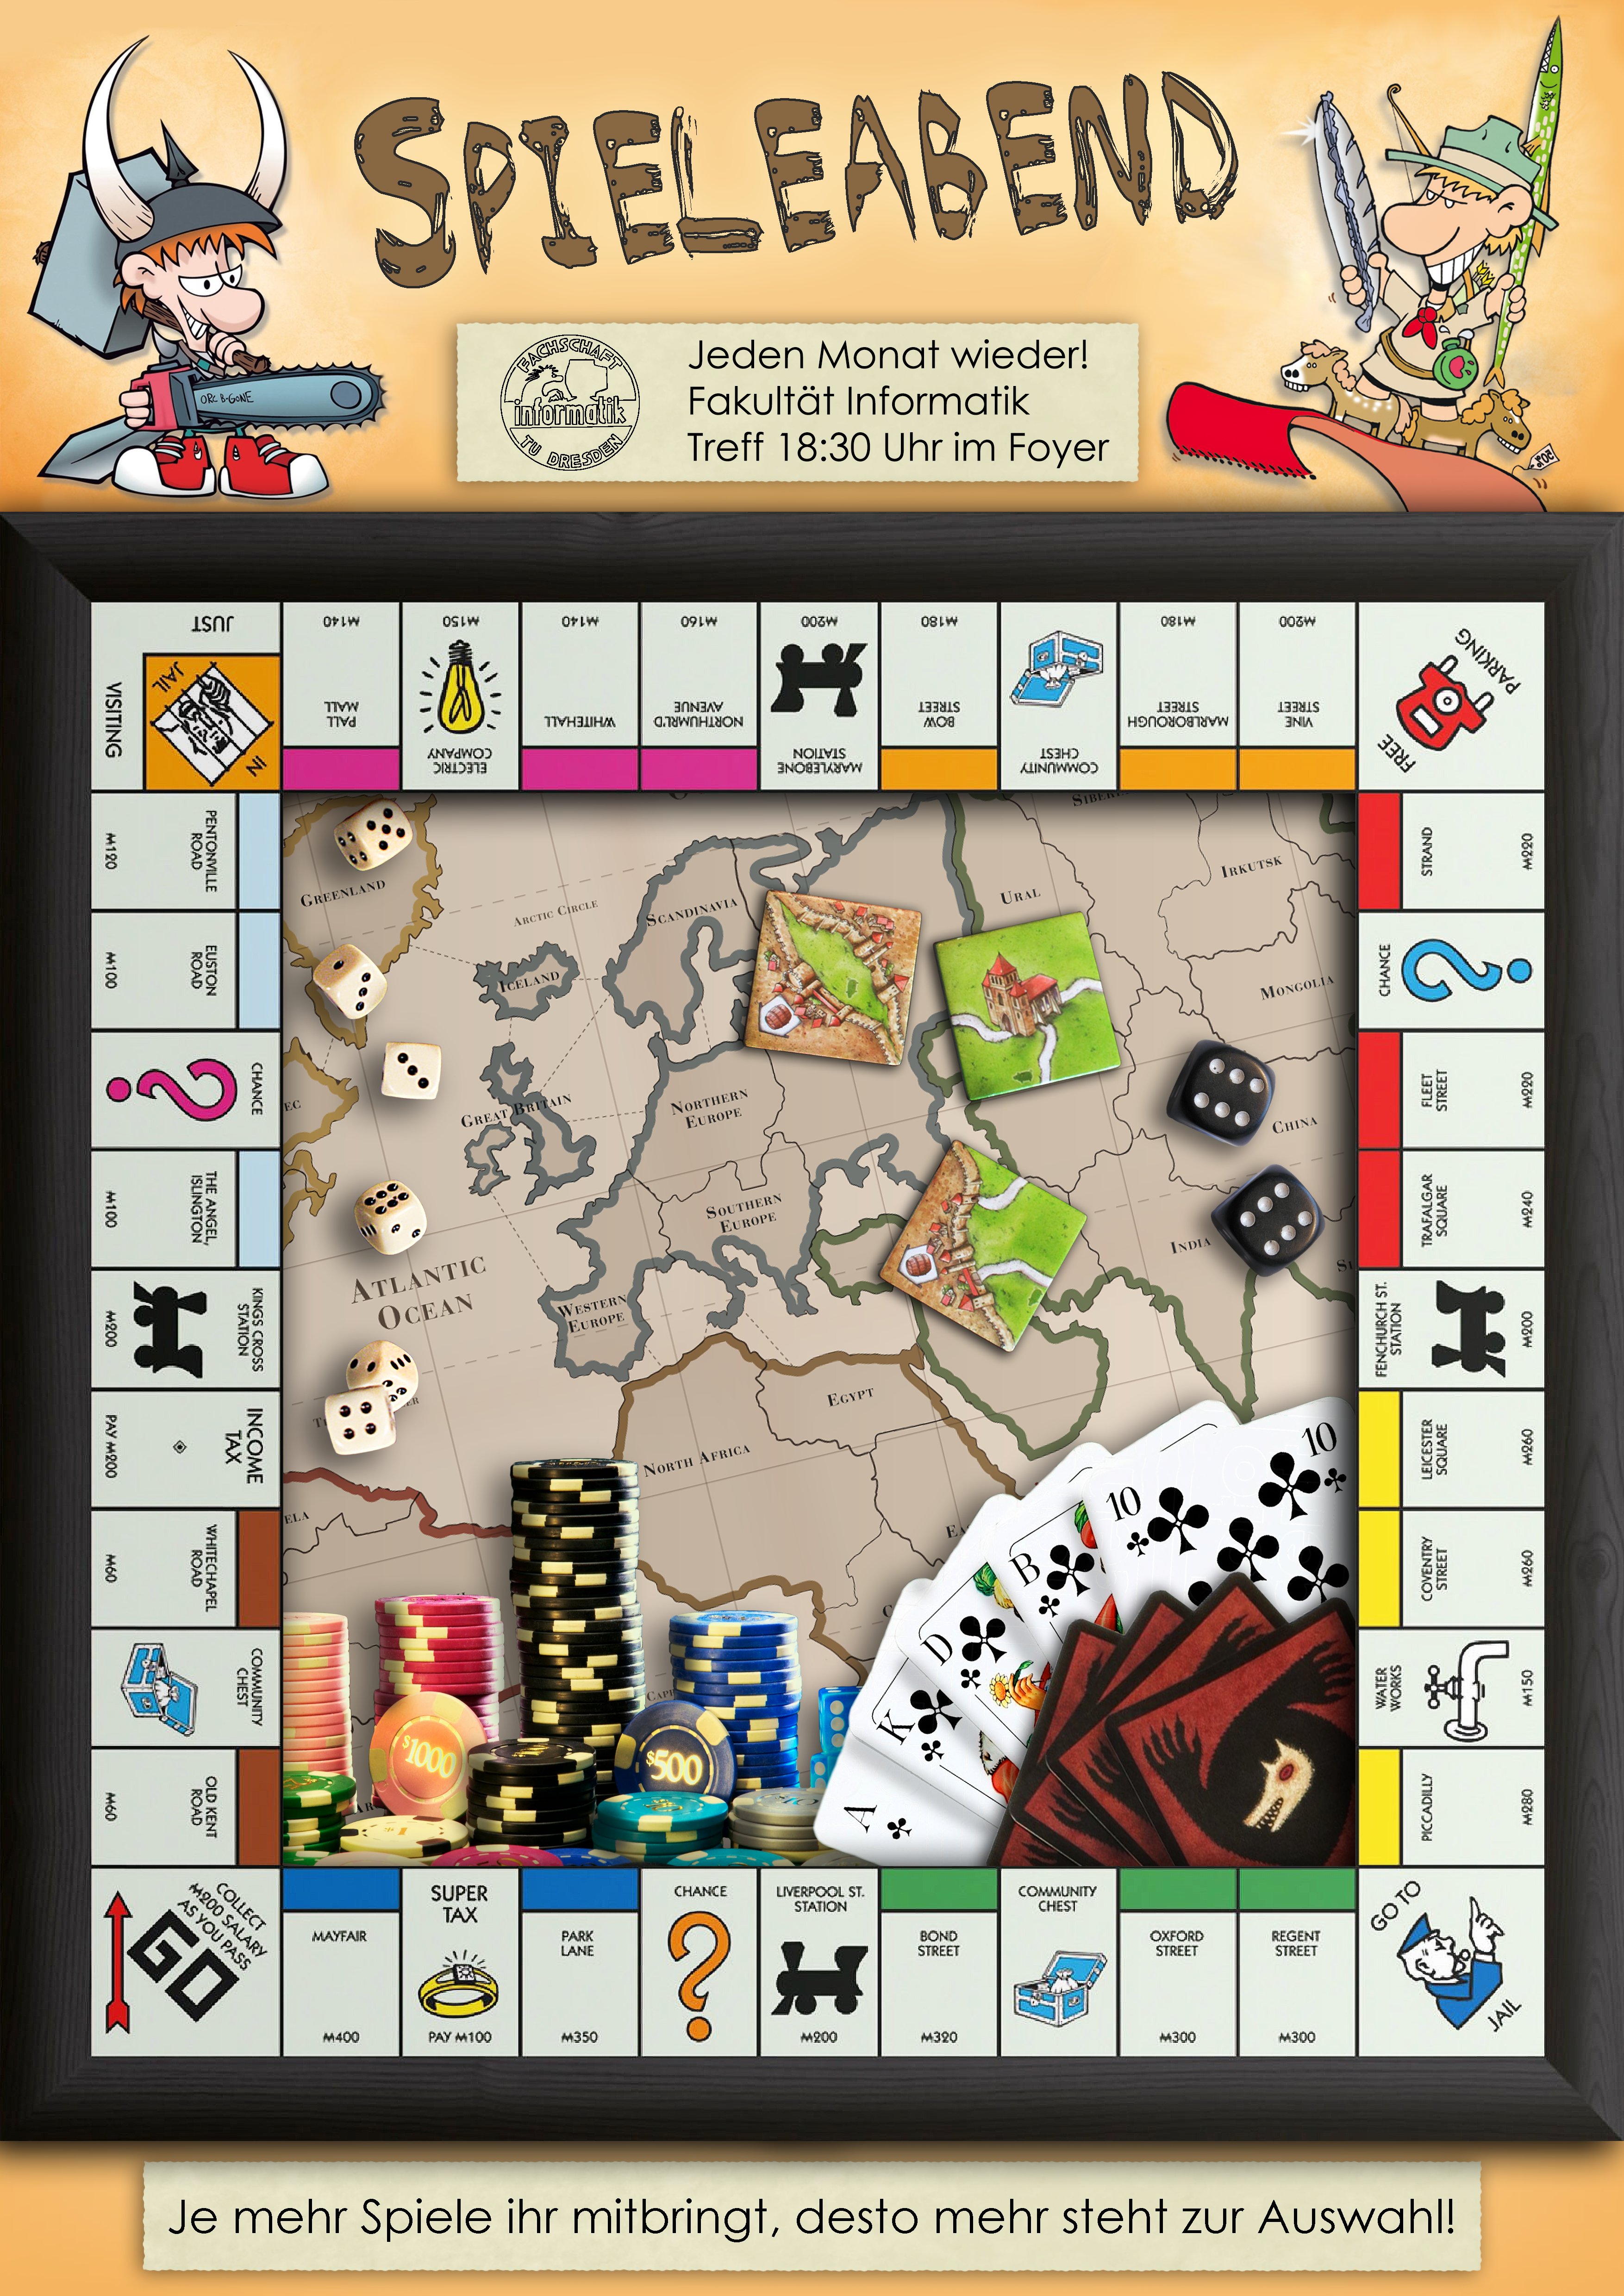
\includegraphics[width=\paperwidth,height=\paperheight,keepaspectratio]{img/spieleabend.png}%
\vfill
}}}
\mbox{}

\addchap{Der Studentenclub Count Down}

%TODO: Lageplan und Bilder vom CD

\begin{wrapfigure}{l}{0.32\textwidth}
  \vspace{-15pt}
  \begin{centering}
    
\includegraphics[width=0.3\textwidth]{img/countdown.jpg}
  \end{centering}
  \vspace{-20pt}
\end{wrapfigure}

Um einen Ort für gemeinsame Treffen und Aktivitäten zu haben, betreiben wir vom Studentenklub IZ e.V. das Count Down.
Dieses befindet sich im Keller des Wohnheims Güntzstraße 22 und liegt damit auf halbem Weg zwischen Campus und Neustadt.
Mit einer Mischung aus gemütlichen Kneipenabenden und verschiedenen Parties begleiten wir dein Studentenleben, selbstverständlich zu studentischen Preisen!

Montags findet unser traditioneller und fast schon nostalgischer Spieleabend statt.
Damit es nicht langweilig wird, haben wir eine große Auswahl an an verschiedenen Brett- und Kartenspielen parat.

Bei den Erasmus-Partys hast du jeden Dienstag die Gelegenheit, gemeinsam mit ausländischen Studenten zu feiern und dere Kulturen kennen zu lernen.

Darüber hinaus gibt es auch viele Veranstaltungen, die nicht im festgeschriebenen Rythmus stehen, aber trotzdem immer wieder stattfinden.
Dazu gehören unter anderem ein Kneipenquiz, Cocktail- und Bowleabende sowie der Metalalterabend.
Den aktuellen Plan findest du auf unserer Internetseite: \url{countdown-dresden.de}.

Du willst gern einmal selbst auf der Bühne stehen?
Ob mit der Blockflöte oder einem spannenden Reisebericht:
Auch dafür ist bei uns Platz im Klub und Kalender!

Und solltest du keine fremden Zuschauer haben wollen, sondern einfach mit deinen Freunden eine Party außerhalb deiner eigenen vier Wände geben, bist du ebenfalls bei uns genau richtig.
An allen Tagen, an denen wir keine Veranstaltung geplant haben (insbesondere am Freitag und Samstag), hast du die Möglichkeit, unseren Klub zu studentisch günstigen Preisen zu mieten, Barpersonal, Aufräumen und Putzen inklusive.
Schau einfach auf unsere Homepage und reservier einen Termin!

Das reicht dir immer noch nicht?
Du möchtest das Studentenleben gern selbst mit gestalten?
Du triffst gerne viele neue, nette Leute?
Du hast vielleicht sogar weitere Ideen für interessante Veranstaltungen?
Du möchtest gern einmal selbst an der Bar stehen und dabei nicht den Chef im Nacken sitzen, sondern den Spaß im Vordergrund stehen haben?
Sprich uns einfach direkt an, neue Mitglieder sind immer herzlich willkommen.

Ob als Gast oder als neues Mitglied - wir freuen uns, dich bald bei uns begrüßen zu dürfen.

\textit{Dein Team vom Count Down}

\addchap{ascii - Das Café in der Fakultät}

\includegraphics[width=\linewidth]{img/ascii.jpg}

Bereits seit 2007 existiert im Gebäude der Fakultät Informatik das ascii, ein Café betrieben von Studenten für Studenten, Mitarbeiter und Besucher, kurzum: für jeden.
Das ascii hat alles was ein richtiges Café so braucht: Kaffee, Kuchen, Bagels so wie alles was Nerds an der Fakultät so brauchen: Koffeinhaltige Kaltgetränke!
Zudem zählt das ascii zu den wenigen Adressen auf dem Campus, in denen man neben Club Mate auch Kolle Mate und Premium Cola erhält.
Hinter dem Tresen stehen Studenten, die gerne an einem Tag in der Woche noch ein paar Stündchen ihrer Freizeit zur Verfügung stellen.

Das ascii wird von einem studentischen Verein betrieben und ist seit seiner Gründung eine zentralen Anlaufstelle für jede und jeden an der Fakultät.
Hier treffen sich Studenten, Mitarbeiter und Professoren um ihre Pausen zu verbringen,
zu arbeiten oder einfach ihren Koffeinhaushalt aufzufüllen.
Auf den gemütlichen Sofas kann man die Zeit wunderbar an sich vorbei streichen lassen,
gemeinsam an Projekten arbeiten, lernen, programmieren oder einfach nur mit seinen Kommilitonen plaudern.
Du kennst noch niemanden an der Fakultät?
Du hast Fragen oder Gesprächsbedarf?
Wenn du ins ascii kommst, wirst du schnell sehen, dass an dem Vorurteil, Nerds seien nicht sozial, absolut nichts dran ist.

Wenn du jetzt Lust bekommen hast, das ascii zu besuchen oder sogar als Mitglied selbst mitzumachen, dann komm doch einfach mal vorbei und sag Hallo!

Weitere Hinweise findest du auf \link{http://www.ascii-dresden.de/}.

\textit{Wir öffnen in der Vorlesungszeit Montag bis Donnerstag von 9 bis 17 Uhr und Freitags von 9 bis 15 Uhr. Dazwischen sind wir aber auch häufig im Café anzutreffen.}

\addchap{ZIH - How To}

%TODO: lustige Bildchen/Cliparts (höhö) um alles aufzulockern?

\minisec{Login}
Das Wichtigste am ZIH ist dein Login.
Mit Benutzername (s-Nummer) und dazugehörigem Passwort hast du Zugang zu nahezu jedem angebotenen Dienst.
Du kannst dich damit von daheim ins Uninetz einwählen und dich in jExam für Übungen einschreiben.
Behandle daher deine Logindaten wie eine Bank-PIN.
Jeder, der Benutzername und Passwort kennt, ist in der Lage, sämtliche Dienste unter deinem Namen in Anspruch zu nehmen, d.h. dich aus Lehrveranstaltungen ein-/auszutragen, E-Mails unter deinem Namen zu verschicken oder unter deinem Namen im Internet zu surfen.
Nachgewiesenermaßen gibt es jedes Jahr ein paar Leute, die allzu leichte Passwörter knacken und dann z.B. veröffentlichen.
Wähle deshalb ein langes, schwieriges Passwort.

\minisec{E-Mail}
Du bekommst vom ZIH zwei E-Mail Adressen:
\textit{s1234567@mail.zih.tu-dresden.de} und einen Alias von der Form \textit{vorname."-nachname@mailbox.tu-dresden.de}.
Falls dein Name an der TU Dresden bereits existiert, lautet die Alias-Adresse für Max Mustermann dann z.B. \textit{max.mustermann1@mailbox...}.
Welche der beiden Adressen du verwendest ist Geschmackssache.
Per Webmail kannst du auf dein Postfach zugreifen.
Empfehlenswert ist es auch, deine Mails an eine persönliche Adresse weiterzuleiten, damit du nichts verpasst.
Ansonsten lassen sich die Mails natürlich auch über IMAP direkt abrufen.
Vor allem E-Mails von der Uni werden an diese Adressen geschickt.
So beispielsweise die Ankündigung der Prüfungseinschreibung oder die Erinnerung an die Rückmeldung für's kommende Semester.
Außerdem werden bei einigen Mailinglisten zu Lehrveranstaltungen nur Adressen von der Domain der TU akzeptiert.

\minisec{Webspace}
Jeder Student hat 100MB Speicherplatz auf den Servern des ZIH, den er frei nutzen kann.
Darunter fallen auch die Benutzereinstellungen für Firefox, Thunderbird und das öffentliche Webverzeichnis.
Von den Uni-Rechnern aus kannst du über das Netzlaufwerk H: auf deine Ordner zugreifen.
Im Allgemeinen kommst du jedoch von außen bequem per SSH auf dein Nutzerverzeichnis.

\minisec{Login via SSH}
Per SSH (Secure Shell) bekommst du die Möglichkeit, dich auf bestimmten Servern des ZIH sicher und verschlüsselt einzuloggen, um so auf der Kommandozeile z.B. auf deinen Slot zuzugreifen oder per X-Forwarding grafische Programme zu starten.
Auch kannst du per SFTP Dateien hoch- oder runterladen.
Im Gegensatz zu OSX und Linux hat Windows keinen direkten Support für Programme wie ssh oder scp eingebaut, daher solltest du dir in diesem Fall direkt PuTTY und WinSCP herunterladen und installieren.
Die Loginserver des ZIH, auf denen du dich per SSH/PuTTY/(Win)SCP einloggen kannst, findest du auf den Seiten des ZIH in der sonst auch sehr hilfreichen Serverübersicht.
Als Benutzername nutzt du wie auch sonst deinen ZIH-Login.
In deinem Userhome findest findest du das Unterverzeichnis public\_html.
Alles, was hier liegt, ist über deinen Webspace verfügbar.
Du musst hier allerdings, entweder per chmod, PuTTY oder WinSCP, für alle hochgeladenen Dateien die Leserechte und für alle Verzeichnisse die Lese- und Ausführrechte setzen.
Zur Erstellung einer eigenen Webseit stehen dir auch PHP und Perl zur Verfügung.
Über einen SSH-Tunnel ist es unter Windows sogar möglich, deinen Slot als Netzlaufwerk einzurichten.
Den zuständigen Samba-Server findest du in der ZIH-Serverübersicht und der Name der Freigabe ist deine s-Nummer.

\minisec{Drucken}
Zum Drucken im FRZ, wie auch im ZIH, benötigst du zunächst einmal eine aufgeladene Ricoh-Karte mit der entsprechenden Nummer (bekommt man in der StuRa-Baracke).
Druckst du ein Dokument mit einem FRZ- oder ZIH-PC auf den Ricoh Drucker/Kopierer, musst du diese Nummer eintippen.
Nun kannst du zu einem beliebigen Drucker gehen, die Karte einstecken und den Druckauftrag abrufen.
Da die Ricoh Geräte nur einfarbige A4 Drucke verarbeiten können, solltest du bunte Druckaufträge, sowie Ausdrucke auf Folie, an die entsprechenden anderen Drucker im Druckerauswahldialog senden.
Diese kannst du ca. einen Tag später beim Operator abholen.

\minisec{Installierte Software}
Nicht auf allen Rechnern des FRZ ist dasselbe Betriebssystem installiert.
Möchte man sich den Weg zum falschen Rechenzentrum ersparen, kann man sich vorher auf der Seite des ZIH informieren.
Standardsoftware wie Firefox, Thunderbird, PuTTY, WinSCP, LibreOffice u.v.m. sind auf jedem Rechner zu finden.

\minisec{Ins Uninetz einloggen}
Auf manche Informationen und Dienste des Uni-Webs kann nur zugegriffen werden, wenn du direkt im Uninetz sitzt.
Es gibt trotzdem ein paar Tricks, wie du dich von einem beliebigen Ort aus ins Uninetz einloggen kannst:
Per SSH kannst du \glqq einen Tunnel bauen\grqq \ und so auf diese Webseiten zugreifen (lies dazu bitte die Manpage von SSH oder die PuTTY Dokumentation über Tunnel).
Ebenso steht eine VPN-Verbindung zur Verfügung.

\minisec{WLAN}
Sowohl auf dem Campus wie auch in den Räumlichkeiten der Fakultät kannst du mit deinem Notebook/Smartphone ins Internet.
WLAN wird sowohl verschlüsselt wie auch unverschlüsselt angeboten.
Für's erste gibt es das \textit{VPN/Web}, verbindest du dich mit diesem wirst du nach dem Aufruf einer beliebigen Webseite auf eine Login-Seite der TU weitergeleitet, auf der du deinen ZIH-Login eingibst.
Du solltest jedoch schnellstmöglich auf das verschlüsselte (WPA-TKIP) \textit{eduroam} wechseln, unter anderem, weil dir dieser Zugang auch an sehr vielen anderen Unis weltweit kostenloses Internet mit deinem TU Dresden Login verschafft.

\twocolumn

\addchap{Glossar}

\textbf{AG DSN} \\
Die AG Dresdner Studentennetz kümmert sich um das Internet in einigen Wohnheimen.
Mithelfer werden laufend gesucht.

\textbf{Anmelden} \\
Alle, die in Dresden heimisch geworden sind, sollten nicht vergessen, sich beim Ortsamt des jeweiligen Stadtbezirkes innerhalb von zwei Wochen anzumelden.

\textbf{APB} \\
Steht für Andreas-Pfitzmann-Bau und ist seit Ende 2014 offiziell der Name der Fakultät Informatik, deren Kürzel bis dahin INF war. Du wirst das alte Kürzel vermutlich noch hier und da antreffen.

\textbf{AQuA} \\
Abkürzung für Allgemeine Qualifikation.
Ist ein Bestandteil deines Studiums.
Genaueres:
Siehe Prüfungs- und Studienordnung.

%\textbf{Assistent} \\
%Wissenschaftlicher Mitarbeiter am Lehrstuhl, meist Doktor.
%Leitet oft Übungen oder Seminare.

\textbf{Auslandsstudium} \\
Etwas, das sich im Lebenslauf immer ganz gut macht, von der Erfahrung und möglicherweise guten Bräune ganz abgesehen.
Nähere Informationen gibt es beim FSR, der Erasmus-Koordinatorin der Fakultät Informatik oder im Akademischen Auslandsamt.

\textbf{Bachelor} \\
Die neuen bundesweit eingeführten Abschlüsse.
Merkmale sind ein im Vergleich zum Diplom kürzeres Studium und die Möglichkeit, aufbauend einen Master zu erwerben. Diese Kombination sollte dann einem Diplom entsprechen, so dass der Bachelor in etwa dem Vordiplom entspricht.

\textbf{BAföG} \\
Zum Thema BAföG gibt es sowohl beim StuRa als auch im Studentenwerk Infomaterial und Anträge.
Beantragt wird BAföG beim BAföG-Amt im Studentenwerk, Fritz-Löffler-Str. 18.
Kümmere dich so schnell wie möglich darum, da frühestens ab dem Antragsmonat gezahlt wird.

\textbf{Belegen} \\
Das Hören einer Vorlesung wird auch als Belegen bezeichnet.
Die im Semester gehörten Vorlesungen können in den Belegbogen auf der Rückseite des Studienbuchblattes, das dir mit dem Studentenausweis zugeschickt wurde, eingetragen werden.
Dieses solltest du im Studienbuch abheften.
% macht das überhaupt irgendwer? :D
% Nein und ich habs mal auf können geändert.

\textbf{Beurlaubung} \\
Auf Antrag gewährt die Uni bis zu zwei Urlaubssemester.
Nutze diese Möglichkeit, falls du z.B. auf Grund von Krankheit oder Auslandsaufenthalt ein Semester frei nehmen musst, damit dir dieses Semester nicht als Fachsemester angerechnet wird.
Achte jedoch auf Bestimmungen zur Höchststudiendauer vor allem im Zusammenhang mit dem BAföG.

\textbf{Bibliothek} \\
Primär von Interesse ist für dich die Universitätsbibliothek (SLUB), die du kostenlos nutzen kannst.
Abgesehen davon stehen dir natürlich auch die Städtischen Bibliotheken Dresdens zur Verfügung.
Allerdings gibt es für diese eine Jahresgebühr von 15\euro{} bzw. 10\euro (Abo).

\textbf{Bücher} \\
Es ist ratsam, nicht direkt zum ersten Semester einen Stapel Bücher zu kaufen.
Besser ist es, sich bei höheren Semestern vorher zu erkundigen, welche Literatur ratsam ist.
Außerdem sollte man sich die Bücher, die von Professoren vorgeschlagen werden, zunächst erst mal in der Bibliothek anschauen.
Angebote für gebrauchte Bücher findest du unter anderem in den Campuszeitungen.

\textbf{Campus} \\
Kerngelände der Uni.

\textbf{Campuszeitung} \\
Die zwei Dresdner Campuszeitungen \textit{ad-rem} und \textit{CAZ} erscheinen ein- bzw. zweiwöchentlich.

\textbf{Club Mate} \\
Das ultimative Kultgetränk unter Hackern dieser Welt und im ASCII erhältlich.
Positiver Nebeneffekt nach dem Genuss von Club Mate ist, dass der hohe Koffeingehalt munter macht/hält.
(Nicht mehr ganz so Geheim-)Tipp:
Auch mal die Dresdner Kolle-Mate im ASCII probieren.

\textbf{Creditpoints} \\
Sammelst du mit dem Bestehen von Modulen.
Die Anzahl gibt an, wie viel Zeit du aufgewendet hast (bzw. haben sollst).

\textbf{DAAD (Deutscher Akademischer Austauschdienst)} \\
Deutschlandweite Anlaufstelle für das Auslandsstudium.

\textbf{Dekan} \\
Der Dekan leitet und vertritt die Fakultät und führt die Beschlüsse des Fakultätsrates aus.
Der gegenwärtige Dekan der Fakultät Informatik ist Prof. Baader.

\textbf{dies academicus} \\
Am \glqq akademischen Tag\grqq\ finden anstelle der Vorlesungen und Übungen andere Veranstaltungen statt.
Er dient dazu, den Studenten die Möglichkeit zu geben, einmal einen Blick in andere Fachbereiche zu werfen.

\textbf{Diplom} \\
Alternativer Studienabschluss zum Bachelor+Master.
Im Wintersemester 2010 wurde ein neuer, modularisierter Diplomstudiengang an unserer Fakultät eingeführt.
Im Gegensatz zum Bachelor+Master bietet dieser ein Nebenfach und ein Praktikumssemester.
Das Diplom berechtigt wie ein Master zur Promotion zum Doktor.

\textbf{DrePunct} \\
Bibliothek am Zelleschen Weg 17 (gegenüber der SLUB), die unter anderem die Bücher des Fachbereichs Informatik beinhaltet.

\textbf{Emeal} \\
Der Emeal (auch Mensakarte) wird gebraucht, um in den meisten Mensen Essen zu bekommen.
Er ist gegen eine Kaution von 5\euro\ und Vorlage der Emeal-Bescheinigung sowie des Personalausweises an den Kassen der Mensen erhältlich.
Zu Beginn des jeweils nächsten Semesters muss der Emeal verlängert werden.
Im Rahmen der ESE wird die Mensakarte aber auch direkt ausgeteilt.

\textbf{Erasmus} \\
Eine europaweite Initiative zum Studentenaustausch.
Siehe auch Auslandsstudium.

\textbf{EVA} \\
Lehrevaluation, gegen Ende des Semesters füllst du in jeder Vorlesung einen Fragebogen aus, um den Dozenten, die Vorlesung und die Übungsleiter zu bewerten.

\textbf{Exmatrikulation} \\
Beim Austritt aus der Hochschule (Studienende/-abbruch, Wechsel der Hochschule) muss man sich exmatrikulieren.
Zwangsweise geschieht dies, wenn man die Höchststudiendauer überschreitet oder vergisst, sich rückzumelden oder notwendige Prüfungen endgültig nicht bestanden hat.

\textbf{Fachschaft} \\
Alle Studenten einer Fakultät. Also auch du.

\textbf{Fachschaftsrat} \\
Gewählte studentische Vertreter einer Fachschaft.
Deine studentischen Vertreter findest du im Raum APB E017.
Der Fachschaftsrat freut sich auch immer über Studenten, die mal vorbeischauen und über Probleme oder Anregungen berichten.

\textbf{Fachschaftsratsitzung} \\
Findet einmal wöchentlich im Fachschaftsrat statt.
Hier werden Aktionen geplant, Angelegenheiten der Fakultät diskutiert und vieles mehr.
Jeder ist dazu herzlich eingeladen!
Termine und Sitzungsprotokolle gibt es auf der FSR-Homepage.
Derzeit:
Jeden Montag 18.30 Uhr im großen Ratssaal (APB 1004).

\textbf{Fakultät} \\
In Fakultäten werden verschiedene Fachrichtungen zu einer Lehr- und Verwaltungseinheit zusammengeschlossen (z.B. Fakultät Informatik, Fakultät Maschinenbau, etc.).

\textbf{Fakultätsrechenzentrum (FRZ, jetzt ZIH)} \\
Das Rechenzentrum in der Informatikfakultät wurde früher von dieser betrieben.
Heute gehört es mit zum ZIH.
Der Rechnerpool bietet dir die Gelegenheit, deine Projekte innerhalb der Fakultät mit der dort zur Verfügung stehenden Software zu bearbeiten.

\textbf{Hochschulsport} \\
$\rightarrow$ USZ

\textbf{Immatrikulationsamt} \\
Zuständig für Aktivitäten wie Immatrikulation, Exmatrikulation und Rückmeldung.
Zu finden im Bürogebäude Strehlener Str. 24, 6. Etage und im Netz \link{https://tu-dresden.de/imma/}.

\textbf{INF} \\
Altes Kürzel der Fakultät Informatik. 
Siehe auch APB.

\textbf{Integrale} \\
Kommentiertes Vorlesungsverzeichnis, in dem alle studium-generale-Veranstaltungen zu finden sind.

\textbf{jExam} \\
Online-Plattform für Studenten.
Hier kannst du dich für Übungen, Seminare, Praktika, Prüfungen, etc. einschreiben und deine Prüfungsergebnisse abrufen.
Zur Einschreibung in der ESE-Woche richtest du deinen Account ein und wir zeigen dir direkt, wie du dich einschreiben kannst.

\textbf{Kino} \\
In Dresden gibt es mehrere Kinos, sowohl wahre Paläste für die unbeschwerte Popcornunterhaltung, als auch kleinere Programmkinos wie beispielsweise das Kino im Kasten, das Kino in der Fabrik oder das Thalia.

\textbf{Klausur} \\
Schriftliche Prüfung zu einer Vorlesung, meist am Ende des Semesters.
Auf dem FTP-Server des FSR \link{ftp://ftp.ifsr.de/klausuren} sind viele Klausuren vergangener Jahre erhältlich (dieses Archiv ist nur aus dem Uninetz erreichbar).

\textbf{Kopieren} \\
An vielen Stellen der Uni stehen Kopierer.
Um sie zu benutzen, braucht man eine Kopierkarte.
Die Karten der Firma Ricoh sind im StuRa (Zimmer 1 bzw. 4) und an verschiedenen Kartenautomaten, die über den Campus verteilt sind, gegen einen Pfand von 5\euro\ erhältlich.
Will man mit den Karten auch drucken, sollte man dies vorher angeben.
Bei Bedarf lässt sich diese dann an den entsprechenden Automaten aufladen.
Eine Kopie kostet 5 Cent.
Zusätzlich hast du die Möglichkeit, im Büro des FSR für geringe Kosten zu kopieren und zu drucken.
Zu guter Letzt hat auch die SLUB ein von der Firma Acribit betriebenes Kopier-/Drucksystem, natürlich auch mit einer eigenen Karte.
Außerdem gibt es auf dem Campus verteilt noch etliche Copyshops.

\textbf{Krankenversicherung} \\
Ab dem 25. Lebensjahr musst du eine eigene abschließen, bis dahin bist du meist über die Familienversicherung deiner Eltern mit abgesichert.
Informiere dich bestenfalls direkt bei deiner Krankenkasse zu diesem Thema.

\textbf{Kryptografie} \\
Mathe, die deine Kommunikation beschützt.
Such' mal nach GnuPG, signiert und verschlüsselt deine E-Mails.

\textbf{Leistungsnachweis, Schein} \\
Muss in einigen Fächern erbracht werden, um zu bestimmten Prüfungen zugelassen zu werden.
Im Gegensatz zu den Prüfungen ist er beliebig oft wiederholbar und meist unbenotet.
Das ist jedoch kein Freibrief zum Durchfallen, da man die Scheine für Klausuren oder die Bachelorprüfung benötigt.

\textbf{LSK} \\
Lehrzentrum Sprachen und Kulturen, s. Seite \pageref{sec:sprachausbildung}.

\textbf{Matrikelnummer} \\
Die Nummer, unter der du an der Uni als Student geführt wirst.
Steht auf deinem Studentenausweis.
Du brauchst sie z.B. bei Klausuren und Prüfungen.
Es ist deswegen günstig, sie auswendig zu wissen bzw. den Studentenausweis immer dabei zu haben.
Letzteres lohnt sich sowieso, da er auch dein Semesterticket ist.
Matrikelnummer bitte nicht mit der sNummer verwechseln.

\textbf{Mensa} \\
Es gibt mehrere Mensen auf dem Campus und an den verschiedenen ausgelagerten Fakultäten.
Im Zuge der allgemeinen Technisierung ist in der Mensa ein bargeldloses Zahlungssystem (Emeal) eingeführt worden.
Wo sich welche Mensa befindet und was es an bestimmten Tagen dort Leckeres zu Essen gibt, kann man auf der Seite des Studentenwerkes in Erfahrung bringen. \link{https://www.studentenwerk-dresden.de/mensen}
Für Smartphones gibt es auch etliche mobile Apps.

\textbf{N.N. (nomen nominandus)} \\
Zu Deutsch:
"(noch) zu nennender Name".
Bedeutet:
der Dozent steht noch nicht fest.

\textbf{No Panic} \\
Dieses Heft.
Ein Eigenname aus historischen Gründen und kein falsches Englisch.

\textbf{Prüfungen} \\
Irgendwann muss da jeder ran.
Hierüber sollte man sich genauestens in der Prüfungsordnung informieren.
Prüfungen können nur begrenzt wiederholt werden.
Wichtig ist natürlich auch die Anmeldung zur Prüfung, diese auf keinen Fall vergessen!
Auch daran denken, zu jeder Prüfung den Perso und den Studentenausweis dabei zu haben!
Prüfungen zu schieben ist auch nur eine begrenzt gute Idee, das holt einen schnell wieder ein.

\textbf{Prüfungsamt} \\
Um zu bestimmten Prüfungen zugelassen zu werden, muss man sich beim Prüfungsamt dafür anmelden.
Eventuell muss man auch Scheine, die für die jeweilige Prüfung Voraussetzung sind, vorzeigen.
Weiterhin kann man hier auch Prüfungsergebnisse erfahren und sich für's Nebenfach einschreiben.

\textbf{Prüfungsordnung} \\
Dort erfährst du, welche Prüfungen und Leistungsnachweise für die Bachelorprüfung benötigt werden und welche Fristen einzuhalten sind.
Diese sollte unbedingt gelesen werden, damit man zumindest weiß, warum man irgendwann plötzlich exmatrikuliert wurde.

\textbf{Prüfungszeit} \\
In den Wochen nach den Vorlesungen wirst du wahrhaftig geprüft.
Prüfungen sollten sechs Wochen vor der Prüfungsperiode im Termin feststehen.
Zu einer Prüfung muss man sich per jExam anmelden.
Abmeldungen (Rücktritte) sind unter bestimmten Voraussetzungen ebenfalls über jExam möglich.

\textbf{Rechtsberatung} \\
Eine kostenlose Rechtsberatung bieten der StuRa (Do 13-14 Uhr, 14-täglich) und der Justiziar des Studentenwerkes an.

\textbf{Rektor} \\
Leitet und vertritt die Universität.
Derzeit Prof. Hans Müller-Steinhagen.

\textbf{Rekursion} \\
$\rightarrow$ Rekursion

\textbf{Rückmeldung} \\
Jeder Student, der im darauffolgenden Semester weiter an der Uni studieren möchte, muss sich im angegeben Zeitraum rückmelden.
Die Rückmeldung erfolgt durch fristgemäße Überweisung des Semesterbeitrags.
Die aktuelle Höhe des Semesterbeitrags wird auf den Webseiten des Immatrikulationsamts bekanntgegeben.

\textbf{Rundfunkbeitrag} \\
Studenten, die nicht zu Hause wohnen, müssen ihren Haushalt anmelden.
Für manche Studenten (z.B. BAföG-Empfänger) besteht jedoch die Möglichkeit, sich von der Gebührenpflicht befreien zu lassen.
Dies ist direkt beim Gebührenservice zu beantragen.
Bedenke auch, dass du rückwirkend mit deinem Einzugsdatum zur Kasse gebeten werden kannst, eine verspätete Anmeldung bringt also keinen Vorteil.

\textbf{Schein} \\
$\rightarrow$ Leistungsnachweis

\textbf{Semesterticket} \\
Wird automatisch mit der Überweisung des Semesterbeitrags bezahlt.
Dein Studentenausweis in Verbindung mit einem gültigen Personalausweis gilt als Fahrschein und ist nicht übertragbar.
Dein Semesterticket gilt auch für den Regionalbahnverkehr in ganz Sachsen.

\textbf{Seminargruppe} \\
Die Studierende des ersten Semester sind in sogenannte Seminargruppen eingeteilt. Hast du dich für eine Seminargruppe entschieden, legt diese deinen Stundenplan und deinen Seminargruppenmentor fest. Die Se\-mi\-nar\-grup\-pe soll dir bei der Organisation deines Studiums im ersten Semester helfen und dir den Übergang von der Schule zur Universität erleichtern. Dazu finden regelmäßige Seminargruppentreffen statt. Bitte nimm daran teil, damit du keine wichtigen Infos verpasst!

\textbf{Service Desk} \\
Bei Fragen und Problemen mit den Computern an der Uni, Logins, E-Mail, WiFi usw. wird dir hier geholfen. Den Service Desk findest du im APB im Zimmer E036.

\textbf{SHKs} \\
Studentische Hilfskräfte werden von den Lehrstühlen als Tutoren oder für wissenschaftliche Hilfstätigkeiten eingestellt.

\textbf{Skript} \\
Manchmal veröffentlicht der Dozent einer Vorlesung ein eigenes Skript, das dann im Netz öffentlich zugänglich ist und ausgedruckt werden kann oder in einem Copyshop gekauft werden kann.
Diese Skripte sind jedoch nur als Gerüst einer Vorlesung anzusehen und reichen nicht für ein selbständiges Eigenstudium aus.
Damit wollen die Professoren verhindern, dass niemand mehr in den Vorlesungen auftaucht.

\textbf{SLUB} \\
Das Hauptgebäude der Sächsischen Landes-, Staats- und Universitätsbibliothek befindet sich am Zelleschen Weg 18 und ist nicht nur wegen seines schönen, ruhigen Lesesaals immer einen Besuch wert.
Dazu gibt es einige Zweigstellen wie den DrePunct.
Zum Ausleihen von Büchern benötigst du einen Bibliothekausweis, den man jederzeit in der Hauptbibliothek beantragen kann.

\textbf{sNummer} \\
Die Nummer, die du für alle Loginvorgänge benötigst.
Steht auf deinem Studienbuchblatt unter \textit{Login-Kennung}.
Du brauchst sie eigentlich immer, zum Beispiel zum Anmelden in jExam oder für den Zugriff auf das Uni-WLAN.
Es ist deswegen günstig, sie auswendig zu lernen.
sNummer bitte nicht mit der Matrikelnummer verwechseln.

\textbf{spiritus rector} \\
Der \glqq leitende Geist\grqq{} wird jedes Jahr von einigen Enthusiasten im StuRa herausgebracht.
In ihm kann man u.a. sämtliche Adressen von Kneipen oder Fachschaftsräten finden. Ab diesem Jahr gibt es ihn nur noch online unter \link{http://spirex.de}.

\textbf{STAV} \\
Die studentische Arbeitsvermittlung bietet eine Liste von aktuellen Jobs an.
Findet man in der StuRa-Baracke oder auf deren Webseite \link{http://www.stav-dresden.de}.

\textbf{Stundenplan} \\
Im ersten Semester hast du mit der Einschreibung in eine Seminargruppe einen festen Stundenplan erhalten. In diesem findest du alle wichtigen Lehrveranstaltungen mit Ort und Zeit versehen. Bitte beachte, dass sich gerade in den ersten Wochen der Stundenplan kurzfristig ändern kann.
Ab dem zweiten Semester musst du dir deinen Stundenplan selbst zusammenstellen.

\newpage

\textbf{Studentenrat (StuRa)} \\
Er vertritt die studentischen Interessen gegenüber der Universität und der Politik und kümmert sich unter anderem um die Verhandlung deines Semestertickets oder um gravierende Probleme mit dem Studentenwerk oder anderen Institutionen.
Außerdem bietet er auch Beratung bei studienrelevanten Problemen (BAföG, etc.) an.
In der StuRa-Baracke befinden sich neben dem Servicebüro des StuRas auch die Büros von STAV und Integrale.

\textbf{Studentenwerk} \\
Fritz-Löffler-Str. 18.
Das Studentenwerk ist zuständig für die Mensen, Studentenwohnheime, BAföG, Beratungen, Wohnungsvermittlung, etc.

\textbf{Studienbuch} \\
In das Studienbuch solltest du deine ausgefüllten Studienbuchblätter zusammen mit erlangten Scheinen abheften.
% Macht das eigentlich überhaupt jemand?
% S.o., aber hier hab ichs mal auf solltest geändert.

\textbf{Studienordnung} \\
Die Studienordnung legt einen Rahmen für den Ablauf eines Studiums fest, z.B. welche Vorlesungen gehört werden sollten.
Studienordnungen kannst du beim Prüfungsamt, der Studienberatung oder beim FSR bekommen.
Außerdem solltest du im Laufe der ESE zusammen mit dieser No Panic eine erhalten haben.
Unbedingt mal lesen, denn sie enthält deine Rechte und Pflichten.

\textbf{studium generale} \\
Freiwilliges Vorlesungsangebot zum über-den-Tellerrand-schauen.
Siehe Integrale.

\newpage

\textbf{SWS (Semesterwochenstunden)} \\
Die SWS sind eine Maßeinheit für die Menge von Vorlesungsstunden, die man pro Semester von einer spezifischen Vorlesung besucht.
2 Semesterwochenstunden entsprechen 90 Minuten (eine \emph{Doppelstunde}) pro Woche in der Vorlesungszeit.
Wenn z.B. im zweiten Semester 3 SWS Mathevorlesungen ausgeschrieben sind, entspricht das jede Woche einer Doppelstunde und zusätzlich alle 2 Wochen noch einmal einer Doppelstunde Mathe.
Bitte beachte bei zweiwöchentlichen Veranstaltungen, in welchen Wochen die Veranstaltung stattfindet. Meistens kann dir der Vorlesende oder dein Übungsleiter weiterhelfen.

\textbf{TUDIAS} \\
TUD Institute of Advanced Studies, s. Seite \pageref{sec:sprachausbildung}.

\textbf{Übungen} \\
Hier wird der Vorlesungsstoff praktiziert.
Es wird von dir als Student erwartet, das Übungsblatt vorher zumindest anzuschauen, um dann die Lösungen zu diskutieren.

\textbf{USZ (Universitätssportzentrum)} \\
Die Universität bietet eine breite Palette von Sportarten zu günstigen Preisen an (normalerweise 15\euro\ pro Semester, je nach Sportart auch mehr).
Welche Sportarten angeboten werden und wie du dich anmeldest, kannst du auf der Webseite \link{https://tu-dresden.de/usz} nachlesen.
Zum Semesterbeginn findet die Einschreibung online statt.
Auf die Termine dafür unbedingt achten, beliebte Kurse sind sehr schnell voll!

\textbf{VL} \\
Vorlesung

\textbf{Wahlen} \\
Gibt es immer im Wintersemester für die Fachschaftsräte der Fakultäten der Uni, die dann Vertreter in den StuRa und in die verschiedenen Gremien entsenden.
Weiterhin können die studentischen Mitglieder des Fakultätsrates gewählt werden.

\textbf{xkcd} \\
Informatiker-Kult-Webcomic auf\linebreak \url{https://xkcd.com}. Du findest einige berühmte xkcd-Comics in diesem Heft.

\textbf{ZIH} \\
Das Zentrum für Informations- und Hochleistungsrechnen.
Es ist zuständig für alles was mit Computern, Logins, E-Mail, WiFi usw. zu tun hat.

%\vfill
%\includegraphics[width=\linewidth]{img/ese2013/tutorium.jpg}

\onecolumn

\renewcommand*{\chapterheadstartvskip}{\vspace{-3em}} % Ist eh die letzte Überschrift.
\addchap{Links}

\scalebox{.7}{
    \begin{tabular}{r p{14cm}}
    \linklist
    \end{tabular}
}

\addchap[Campusplan]{}
\thispagestyle{empty} %keine Seitenzahl
\AddToShipoutPicture*{\put(0,0){%
\parbox[b][\paperheight]{\paperwidth}{%
\vfill
\centering
\adjincludegraphics[height=\pageheight,keepaspectratio,trim={0 0 {.5\width} 0},clip]{img/campusplan_highlighted.pdf}%
\vfill
}}}
\mbox{}
\newpage
\thispagestyle{empty} %keine Seitenzahl
\AddToShipoutPicture*{\put(0,0){%
\parbox[b][\paperheight]{\paperwidth}{%
\vfill
\centering
\adjincludegraphics[height=\pageheight,keepaspectratio,trim={{.5\width} 0 0 0},clip]{img/campusplan_highlighted.pdf}%
\vfill
}}}
\mbox{}

\thispagestyle{empty} %keine Seitenzahl
\AddToShipoutPicture*{\put(0,0){%
\parbox[b][\paperheight]{\paperwidth}{%
\vfill
\centering

\includegraphics[height=\pageheight, width=\pagewidth]{img/filmwerbung.pdf}
\vfill
}}}
\mbox{}

\newpage
\thispagestyle{empty} %keine Seitenzahl
\color{white}

\begin{minipage}[t][\textheight][b]{.60\textwidth}
\footnotesize
\textbf{Herausgeber} \\
Fachschaftsrat Informatik der TU Dresden\\
Nöthnitzer Straße 46\\
01187 Dresden\\[1\baselineskip]

Alle verwendeten Comics von Randall Munroe (\textit{xkcd.com}) unter Creative Commons Lizenz:\\
\url{https://creativecommons.org/licenses/by-nc/2.5/}\\[1\baselineskip]

Redaktionsschluss dieser Ausgabe ist ein warmer Sommermorgen Anfang September 2016.\\[1\baselineskip]

Mitarbeit an der nächsten Version,\\
Verbesserungsvorschläge oder Tippfehlerfunde\\
sind unter \url{https://github.com/fsr/nopanic}\\
immer willkommen!\\[1\baselineskip]

Powered by \LaTeX
\end{minipage}%
\hspace{.20\textwidth}%
\begin{minipage}[t][\textheight][b]{.01\textwidth}
\scalebox{.63}{
\begin{minipage}[b][\textheight][b]{11em}
\raggedleft
\textbf{Dank an:}\\[1\baselineskip]
Alexander Lichter\\
Alexandra Krien\\
Amelie Wagner\\
Andreas Geyer\\
Andrey Ruzhanskiy\\
Anita Grützner\\
Axel Reinicke\\
Bettina Groschopp\\
Christian Kabelitz\\
Christoph Kepler\\
Dennis Dimov\\
Dirk Legler\\
Fabian Horn\\
Felix Döring\\
Felix Wittwer\\
Franziska Ressel\\
Ian Alexander List\\
Jan-Erik Wieczorek\\
Janek Speit\\
Janine Ahnert\\
Jasmin Delling\\
Jens Wettlaufer\\
Julius Gonsior\\
Justus Adam\\
Katharina Letz\\
Katja Linnemann\\
Kilian Költzsch\\
Landfried Kraatz\\
Lars Engeln\\
Louis Wilke\\
Lucas Vogel\\
Lukas Haack\\
Manuel Thieme\\
Marc Kandler\\
Marc Satkowski\\
Marc-Eric Schneider\\
Martin Welcker\\
Marvin Arnold\\
Max Korn\\
Max Langer\\
Max Maier\\
Maximilian Kindt\\
Michael Schneider\\
Patrick Teufert\\
Paul Genssler\\
Paul Hoffmann\\
Philipp Heisig\\
Richard Kwasnicki\\
Richard Mörbitz\\
Robert Glöckner\\
Robert Peine\\
Sam Toorchi Roodsari\\
Sandra Kukulka\\
Sascha Peukert\\
Sebastian Mielke\\
Sebastian Rottmann\\
Sebastian Vogt\\
Severin Engert\\
Simon Hanisch\\
Stephan Fischer\\
Stephan Kirst\\
Sven Springer\\
Thanh-Tien Tenh Cong\\
Tobias Hänel\\
Vincenz Herz
\end{minipage}
}
\end{minipage}

\enlargethispage{2\baselineskip}

\newcommand\BackcoverPic{%
\put(0,0){%
\parbox[b][\paperheight]{\paperwidth}{%
\vfill
\centering

\includegraphics[width = \paperwidth, height = \paperheight]{cover/Hinten}%
\vfill
}}}
\AddToShipoutPicture*{\BackcoverPic}


\end{document}
